\chapter{When do the effects of interaction happen? Interacting and disturbed galaxies in the COSMOS field}\label{chapter3}

%%%%%%%%%%%%%%%%%%%%%%%%%%%%%%%%%%%%%%%%%%%%%%%%%%

%%%%%%%%%%%%%%%%% BODY OF PAPER %%%%%%%%%%%%%%%%%%

\section{Introduction}\label{introduction}
\noindent To fully map out the effect of galaxy interaction, we must understand its impact through various merger histories and across the full dynamical timescale of the interaction. The dynamical timescale is the full time of the interaction, from the two galaxies approaching each other to flying by and escaping or merging. We cannot observe a full, continuous interaction and have to rely on many observations to provide snapshots of the dynamical timescale we can piece together. This, however, makes it difficult to conclusively find link the dynamical timescale to physical processes. Often, observational samples are too small to be fully representative or deep studies of individual systems are required to identify the dynamical timescale \citep{2000ApJ...530..660B, 2012A&A...539A..45L, 2014A&A...567A.132W}. We gain insights from works focused on simulations, where the dynamical timescale can be directly recorded. They find sudden increases in star formation occurs at the mid-point of the dynamical timescale, as the two systems flyby \citep{2008MNRAS.384..386C, 2019MNRAS.490.2139R, 2021MNRAS.503.3113M}. However, confirming this observationally remains elusive \citep{2023ApJ...958...96R}. Observational confirmation is also difficult with nuclear activation and quenching of interacting systems \citep{2011MNRAS.418.2043E, 2018PASJ...70S..37G, 2023ApJ...942..107S}. 

While cannot directly measure the full dynamical timescale for individual systems, we can create large samples of interacting galaxies contain systems spanning the full dynamical history. Attempts to create such a sample have been either by machine learning classification \citep{2019A&A...626A..49P, 2023A&A...669A.141S}, visual classification by citizen scientists \citep{2010MNRAS.401.1043D} or by photometric parameterisation \citep{2004AJ....128..163L, 2023MNRAS.522....1N}. However, as stated previously, each sample has always been plagued by contamination and a loss of statistical significance when broken down into stages.

An alternate approach to directly measuring the dynamical timescale of an interaction has been to infer it from the projected separation between the two systems. Early works showed that there was significant star formation enhancement (SFE) in galaxy pairs with small separations \citep{2003MNRAS.346.1189L,2008MNRAS.385.1903L, 2008AJ....135.1877E, 2022ApJ...940....4S}. A connection was also found between the projected separation in galaxy pairs and the AGN fraction where, once again, the AGN fraction appears to increase with decreasing projected separation \citep{2009MNRAS.399.2172R, 2011MNRAS.418.2043E, 2017MNRAS.465.2671G, 2021ApJ...909..124S}. However, using projected separation as a proxy for the stage in dynamical time of an interacting history overlooks which part of the dynamical history the interaction is. For instance, if a galaxy pair is found to have small projected separation, without visually confirming the morphology, it is difficult to ascertain if the galaxies are just approaching each other or have just passed each other. Extended morphological tracers can help break this degeneracy, which is critical to our understanding of the effects of interaction.

In this Chapter, we split our large sample of interacting galaxies found in Chapter \ref{chapter2} into four specific stages based on their morphology. Each stage is designed to capture different parts of the dynamical time of an interaction. The stages range from galaxies being close pairs, to overlapping and disturbed, to disturbed and distinct to finally coalescing. This follows the classification methods of developing algorithms for staging of interaction\citep{2019MNRAS.490.5390B,2022ApJ...937...97C}. 

We focus here on the subset of our sample in the Cosmic Evolutionary Survey (COSMOS) survey\footnote{DOI: \href{https://www.ipac.caltech.edu/doi/irsa/10.26131/IRSA178}{10.26131/IRSA178}}. This provides us with ancillary data which contains many galactic parameters of interest and we explore how they evolve with our defined stages of interaction. We primarily focus on the evolution of the stellar masses, star formation rates and AGN classification from various COSMOS catalogues. We use the photometric redshifts available from COSMOS to confirm a set of interacting galaxies and close pairs to draw on trends with projected separation.

This Chapter is laid out as follows in Chapter \ref{data} we briefly summarise the COSMOS catalogue, and describe the process of catalogue matching especially focused on accurate de-duplication and cross-matching. Chapter \ref{method} describes the methods by which we split the interacting systems into stages, and how we identify the secondary galaxies in each pair. In Sections \ref{results:SF_stage} and \ref{results:AGN_stage} we show our results of star formation and active galactic nuclei evolution with interaction stage and present an initial discussion. These are followed in Chapter \ref{discussion} where we compare to previous works and put our results in the context of the field. Finally, in Chapter \ref{conclusion} we make concluding remarks and discuss future work to better our constraints. 

\section{Data: Catalogue Matching \& Secondary Identification} \label{data}
\subsection{The COSMOS2020 Catalogue}
In the COSMOS survey, there are multiple catalogues of galactic parameters such as star formation rates (SFR), stellar masses and line emissions. We elect to specifically use the COSMOS2020 catalogue \citep{2022ApJS..258...11W}. This catalogue has a wealth of ancillary information approximately 1.7 million sources in a 2 square degree area of the sky. Each source has been analysed with well known astronomical software (for our purposes, primarily \texttt{\texttt{LePhare}} \citep{1999MNRAS.310..540A, 2006A&A...457..841I}, \texttt{\texttt{EAzY}} \citep{2008ApJ...686.1503B} and \texttt{\texttt{FAST}} \citep{2017MNRAS.465.3390A}). These provide estimates of the physical parameters of each source based on its measured broadband photometry. For our purposes, the parameters of interest are the stellar masses and the estimated star formation rates of each source. For the stellar mass we use the best fit \texttt{LePhare} measurement and for the star formation rates we use the best fit \texttt{EAzY}/\texttt{FAST} measurements. We compare the output masses and SFRs for our sources in Figure \ref{fig:difference-measures}. As shown, there can be wide scatter and disagreement between the two algorithms. We tested different combinations of \texttt{EAzY} and \texttt{LePhare} stellar masses and SFRs to find which would be best to use in this work. We found that using the same algorithm in both parameters revealed the degeneracies of using discrete templates to fit the broad band photometry in the underlying parameter space. Therefore, we elect to inter-mix the algorithms and use the best fit \texttt{LePhare} stellar mass and best fit \texttt{EAzY} SFR measurement.

\begin{figure}
\centering
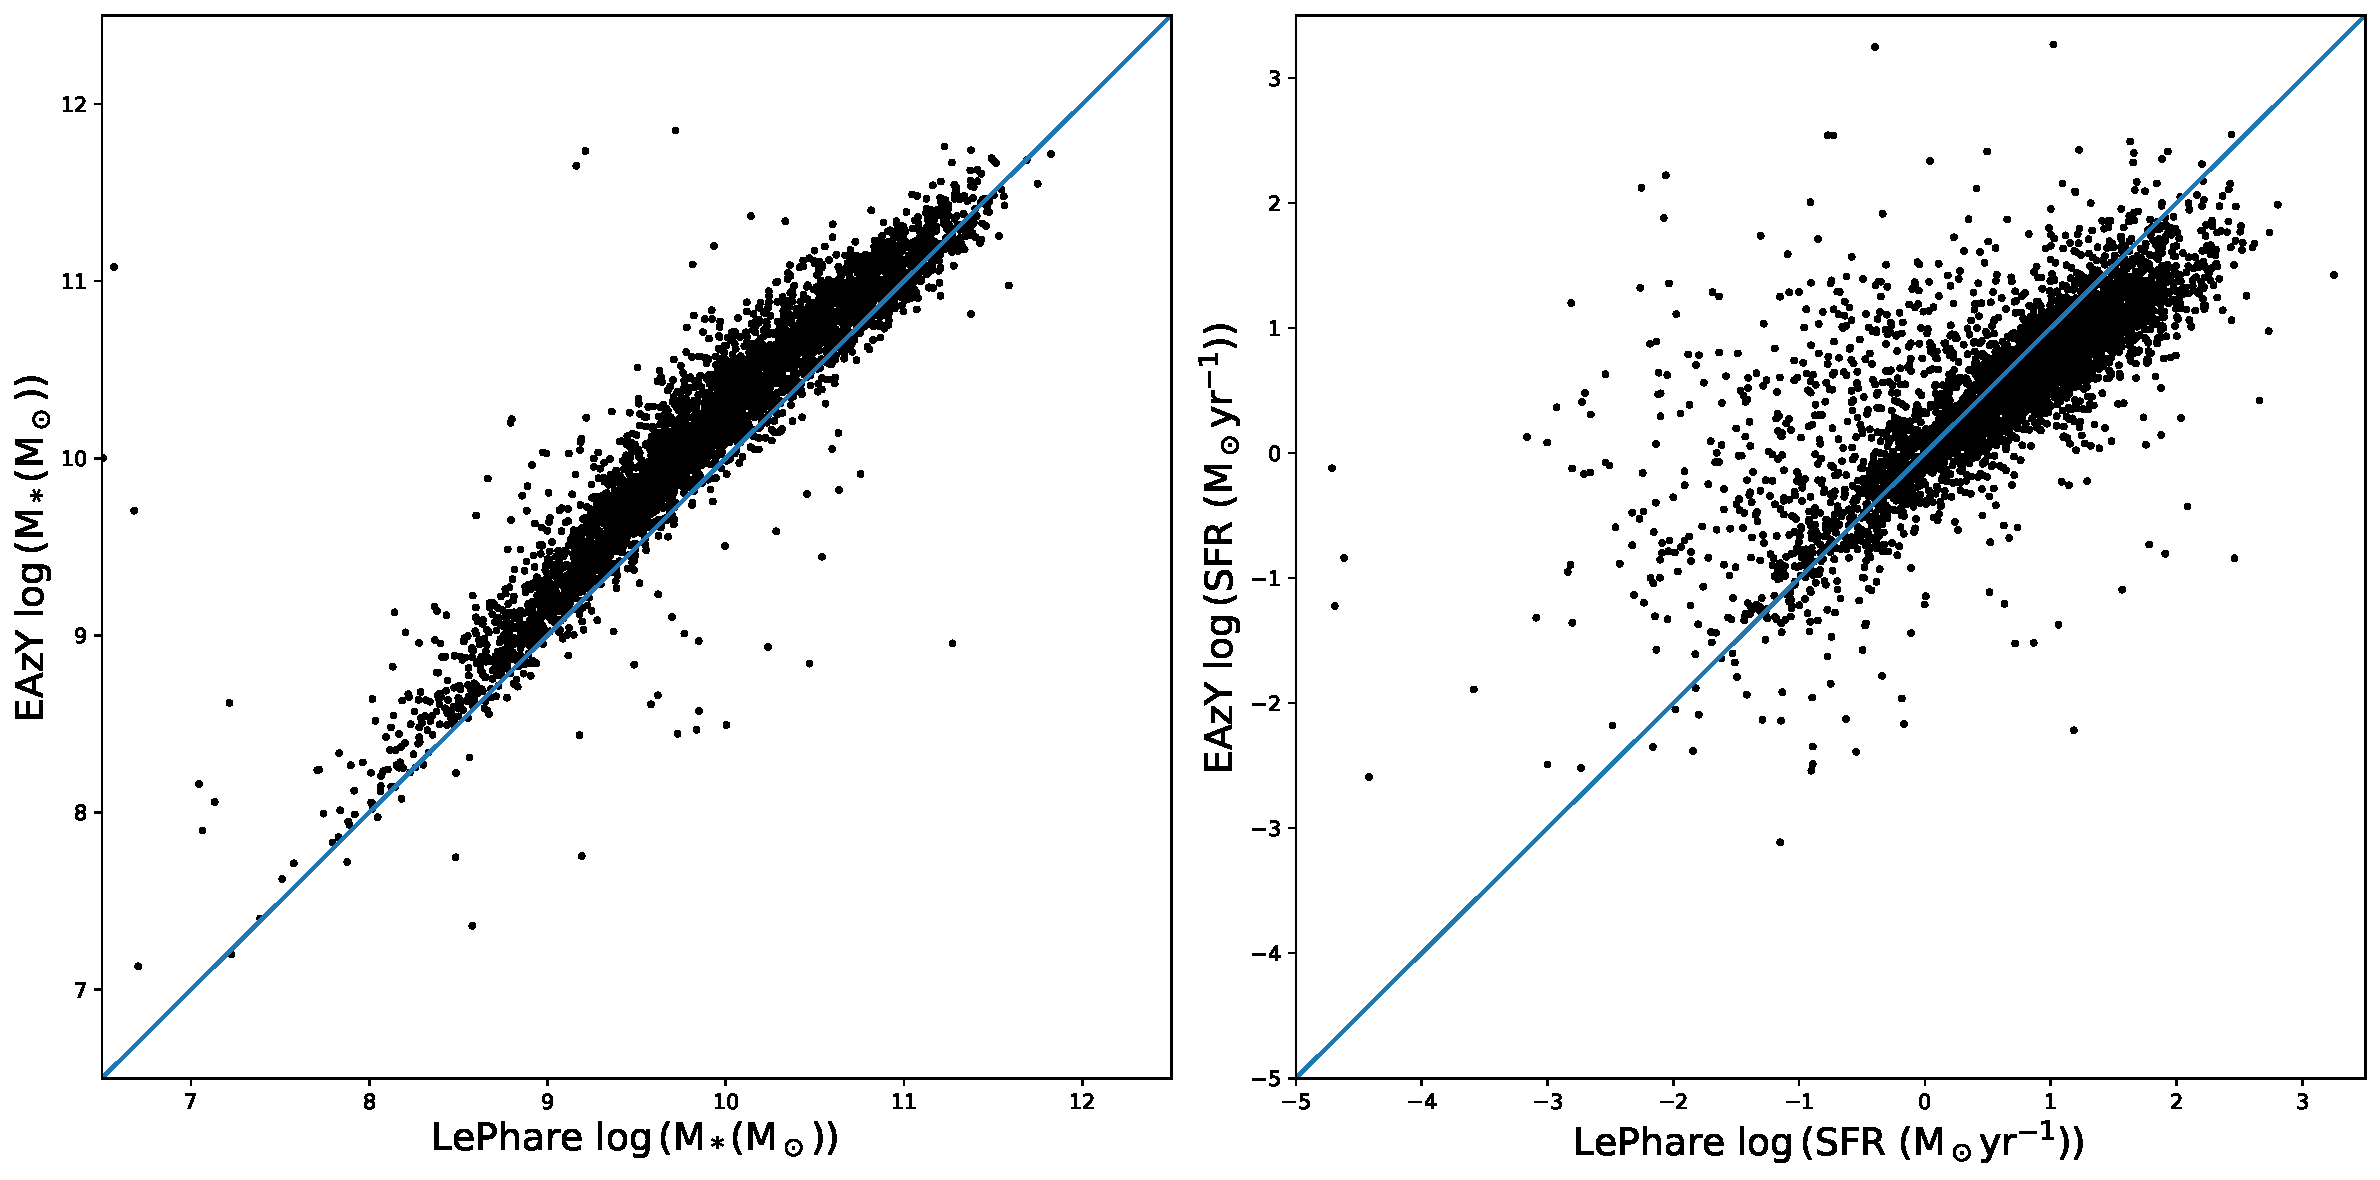
\includegraphics[width=\textwidth]{Chapter3/figures/mass-sfr-scatter.pdf}
\caption[Comparison of the measures of stellar mass and SFR using either \texttt{LePhare} or \texttt{EAzY}/\texttt{FAST} photometric codes to calculate them.]{Comparison of the measures of stellar mass and SFR using either \texttt{LePhare} or \texttt{EAzY}/\texttt{FAST} photometric codes to calculate them. If the algorithms agreed perfectly, the sources would lie on the blue 1:1 line. \textit{Left}: The scatter in the stellar masses between softwares. As shown, \texttt{EAzY} often seems to find larger stellar masses when compared to \texttt{LePhare}. \textit{Right}: Scatter in SFRs when measured with \texttt{LePhare} or \texttt{EAzY}.}
\label{fig:difference-measures}
\end{figure}

Our sample of interacting galaxies has been de-duplicated, but the COSMOS2020 catalogue is not specifically a de-duplicated merger catalogue. We cross match between our sample and the COSMOS2020 catalogues using a position search within $10^{\prime\prime}$ of our sample coordinates. Once we have identified the nearest COSMOS2020 source for each interacting galaxy ID, we de-duplicate based on COSMOS2020 ID and redo the coordinate matching process with any duplicate matches. If no further COSMOS2020 sources were within 10" of the source, then we classify the source as not in the COSMOS2020 catalogue. We find 3,786 of the our sources exist in the COSMOS2020 catalogue.

Once matched, we remove any sources with non-physical photometric measurements for the stellar mass or star formation rates. We then further reduce our sample by only keeping sources within a mass range of $6.5 \leq \log_{10} \text{M}_{*}(\text{M}_{\odot}) \leq 12.5$ and a star formation rate range of $-5 < \log_{10} \text{SFR} (\text{M}_{\odot}\text{yr}^{-1}) \leq 3.5$. We also opt to institute a redshift cut of $z \leq 1.2$. Beyond this redshift, we find that identification of tidal features becomes difficult due to surface brightness dimming and we risk mis-identifying the stages of the interacting galaxies. This also matches the redshift cut applied to the environment catalogue we cross match with in Chapter \ref{data:environ}. Applying these cuts reduces our sample size to 3,689 interacting galaxies.

\subsection{Secondary Identification}\label{sec:sec-ident}
\noindent As the catalogue described in Chapter \ref{chapter2} only contains source coordinates and IDs, we must also manually identify the secondaries of many of our interacting systems. To find the secondaries, we apply three steps. First, a cutout surrounding each source was created. These cutouts were from the COSMOS cutout service, selecting HST-ACS tiles in the $F814W$ filter. Each cutout had a 30" radius (corresponding to 1001 $\times$ 1001 pixels). The original cutout from Chapter \ref{chapter2} was also displayed next to the enlarged cutout. We annotate each cutout with each sources COSMOS2020 ID and measured photometric redshift and error. By annotating each cutout with the sources photometric redshift and ID, we visually assessed each cutout and gave one of the four following classifications to each: system disturbed but secondary could not be identified; secondary could be identified; cannot confirm galaxy is interacting; null redshift (0 or NaN); incorrect primary assigned. 

To associate a secondary galaxy for each primary, the galaxy had to be within the cutout we were visually assessing and within the recorded error of the primary photometric redshift. Using photometric redshift cutoffs in this way is often done when calculating environment parameters \citep[e.g][]{2006MNRAS.373..469B} or defining interacting galaxies by close pairs \citep[e.g][]{2022ApJ...940....4S}. A null redshift is defined as outwith our redshift limits, 0 or NaN. A minority of the cutouts we visually assessed were found to have the incorrect primary at the centre. In these cases, we record the correct primary galaxy ID and extract the ancillary data from the COSMOS2020 catalogue. We then attempted to find the secondary galaxy again for the corrected primary.

Using these definitions, we find that of the 3,689 original systems cross-matched with COSMOS2020 2,283 could not have their secondary identified, 834 had a clear secondary, 446 could not be reliably classified as an interacting galaxy, 248 had a null redshift and 149 were the incorrect primary. Figure \ref{fig:secondary_selection} shows an example of each of our classifications. Each secondary we identify was added to our sample, increasing our sample size to 3,829.

\begin{figure*}
\centering
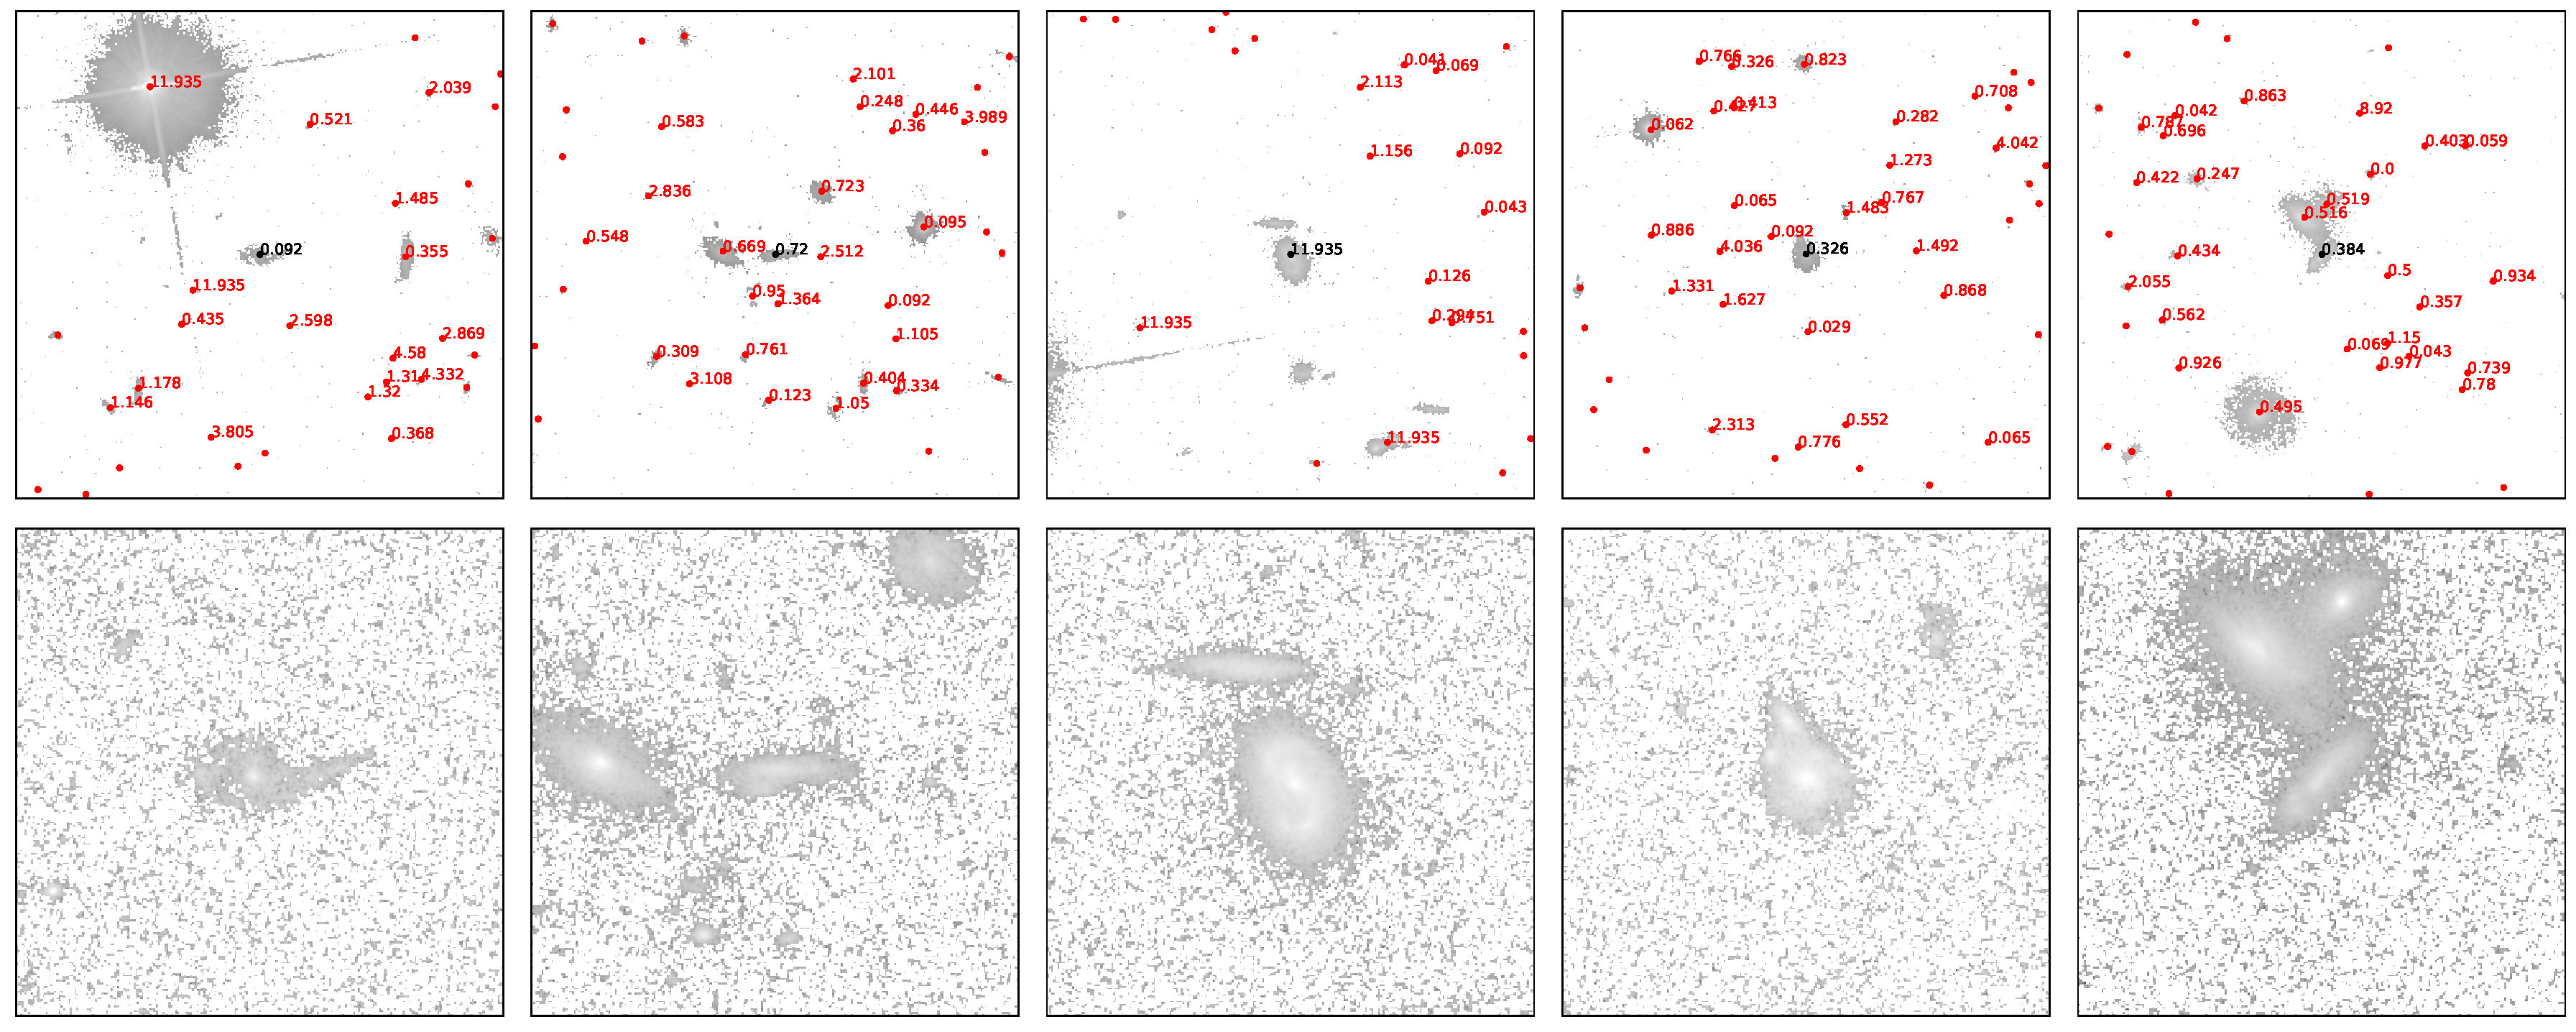
\includegraphics[width=\textwidth]{Chapter3/figures/cutouts_ex.pdf}
\caption[An example of each visual classification made on the cross matched sample.]{An example of each visual classification made on the cross matched sample. These are: (A) where the secondary could not be identified, (B) the primary had a clear secondary, (C) the primary could not be reliably classified as an interacting galaxy, (D) the redshift was null and (E) the incorrect primary was identified. Based on these classifications, we either add the secondary galaxies to the sample or we remove the contamination from it. These images are 30" across using the COSMOS cutout service, selecting HST/ACS tiles as the basis for the observations in the $F814W$ filter.}
\label{fig:secondary_selection}
\end{figure*}

% Define our classifications above.
While initially surprising that the majority of our systems could not have a secondary identified, we found that it was mostly due to limitations in the COSMOS catalogue or the way in which we conduct our secondary identification. Each potential secondary must have a COSMOS ID associated with it, however, when two systems are very close together and small enough they were identified under a single COSMOS ID despite being two separate systems. The same also occurred when two systems were merging or interacting. The tidal features connecting the systems or coalescing systems would only be identified under one ID in the catalogue. Figure \ref{fig:secondary_selection} panel C) shows an example of two systems being close enough together that they have been identified under a single COSMOS2020 entry. Figure \ref{fig:secondaries_found} shows this disparity with the different types of interaction we observe.

\begin{figure}
\centering
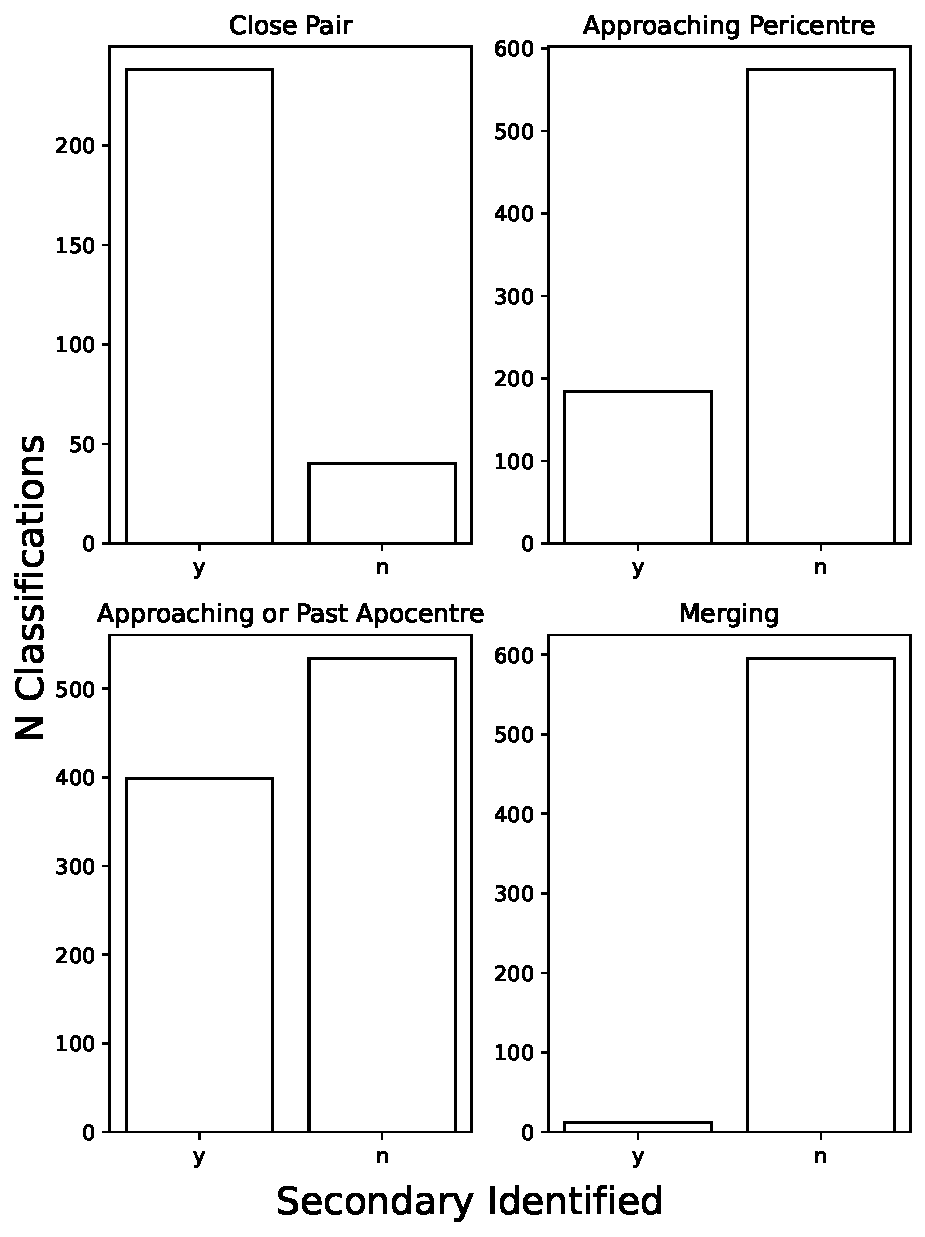
\includegraphics[width=0.95\textwidth]{Chapter3/figures/visualisation_classification.pdf}
\caption[Where a secondary could be identified at different stages in the interaction.]{Where a secondary could be identified at different stages in the interaction. The reasoning for such disparity in secondaries identified is due to the relative distance each the secondary would be from the primary at each stage. For a close pair, we often found the secondary galaxy, but a minority of these were so close together that the entire system was given a single COSMOS ID. The same was true for those interacting systems approaching pericentre or merging. When the secondary was near apocentre, often it would be outside the cutout we were using for visual classification.}
\label{fig:secondaries_found}
\end{figure}

Those galaxies which were found to be contamination (i.e., could not be reliably classified as interacting as they showed little tidal distortion or had no neighbouring systems at a matching redshift or having a redshift of 0) were removed from our sample. Galaxies that could not be reliably classified as interacting were also removed. These systems were often overlapping but at different redshifts, or were systems with irregular morphologies of spiral arms or a clumps were present. There was also many systems that were at high redshift ($z > 1$) where the resolution of the cutouts meant that features could not be discerned visually.

Our final classification type was that the incorrect galaxy had been identified as the primary galaxy. This was the case for 149 systems. These were systems where the interacting galaxies were clearly in the cutout but some tidal debris or some nearby system had been matched from COSMOS. We reassign these systems to the correct COSMOS IDs and then take them through the secondary identification process.

By the end of this selection method, we find a sample size of 3,829 interacting galaxies. We conduct a de-duplication based on the COSMOS2020 ID, which reduces the sample back down to 3,547 interacting galaxies. The remaining systems are each visually confirmed interacting and disturbed galaxies based on their morphology and photometric redshift as measured in the COSMOS2020 catalogue.

For each galaxy in our sample, we define a mass- and redshift-matched control galaxy to investigate differences in their galactic parameters. We find these control galaxies from the COSMOS2020 catalogue. All galaxies within 0.01 dex of our samples stellar mass are selected from the catalogue, and within a $\pm0.01$ redshift slice. We then define the control galaxy as the system furthest from our interacting galaxy. Each control galaxy is then visually confirmed to be non-interacting and have no nearby pairs. We also confirm that it does not already exist in the catalogue, and ensure there is no duplication in the control sample. Figure \ref{fig:matched-distributions} shows the mass distribution of our paired sub-sample of galaxies and their control, showing a mass distribution which is approximately the same as the interacting sample. With the previously defined cuts, we find a control galaxy for all but one of our interacting galaxies.

\begin{figure}
\centering
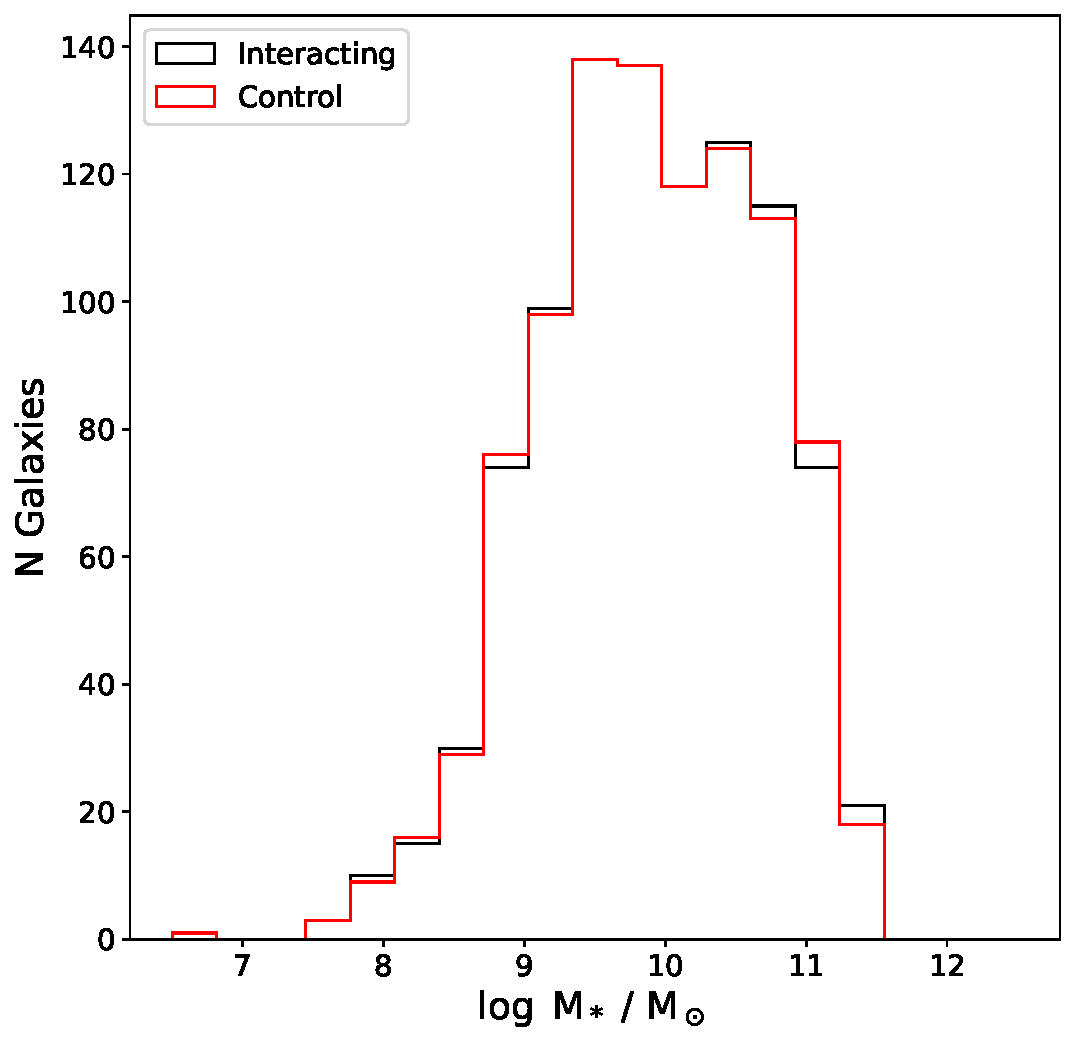
\includegraphics[width=\textwidth]{Chapter3/figures/mass-matching-pairs.pdf}
\caption[The mass distribution of the paired interacting galaxy sample and the control sample.]{The mass distribution of the paired interacting galaxy sample and the control sample. Both primary and secondary galaxies are within this distribution.}
\label{fig:matched-distributions}
\end{figure}

\subsection{Finding Additional Systems}
\noindent As a result of using visual classification to find the secondary galaxy in each interaction, we were able to also confirm other interacting systems which had not been found in our catalogue. Primarily, these extra interacting galaxies are from systems which had more than two galaxies involved in the interaction. Our selection process was built to only find a primary and secondary galaxy and, therefore, we add these extra systems into our sample manually. Other interacting galaxies that were added were low redshift systems which would have appeared to completely fill the cutout of the classification process in Chapter \ref{chapter2}. By looking at the larger COSMOS2020 cutouts, we are able to recover these galaxies and add them to this sample.

In total, we found an extra 841 interacting systems that we could add to our sample. Upon conducting a de-duplication of these with the sample already found, this was reduced to 634 interacting systems. This gives us a total flux-limited sample size of 4,181.

\subsection{Creating the Mass-Limited Sample}
\noindent We now investigate the distribution of our sample between mass and redshift. Figure \ref{fig:redshift_selection} shows the resultant distribution from our flux limited sample. In order to ensure that our results are not biased by a redshift-dependent mass/luminosity limit, we institute a cut in the mass of the interacting systems. Thus, creating a mass limited sample. We elect to use a mass cut of $\log(\frac{M}{M_\odot}) \geq 9.25$, shown by the blue dashed line in Figure \ref{fig:redshift_selection}. This specific cut is motivated by two reasons. First, this is the lowest mass system which is still observed in our the coalescing sample at $z = 1.2$. The second reason is that such a mass cut is approximately the one made in the environment catalogue we will describe later in Chapter \ref{data:environ}. There we make a cut of $\log(\frac{M}{M_\odot}) \geq 9.6$, we find that decreasing the mass cut to $\log(\frac{M}{M_\odot}) \geq 9.25$ does not make major differences to our results. Thus, we opt to use a lower mass cut to increase the number of galaxies in our sample. Making such a cut reduces our flux-limited sample of 4,181 to a mass-limited sample of 3,384 interacting galaxies.

\begin{figure}
\centering
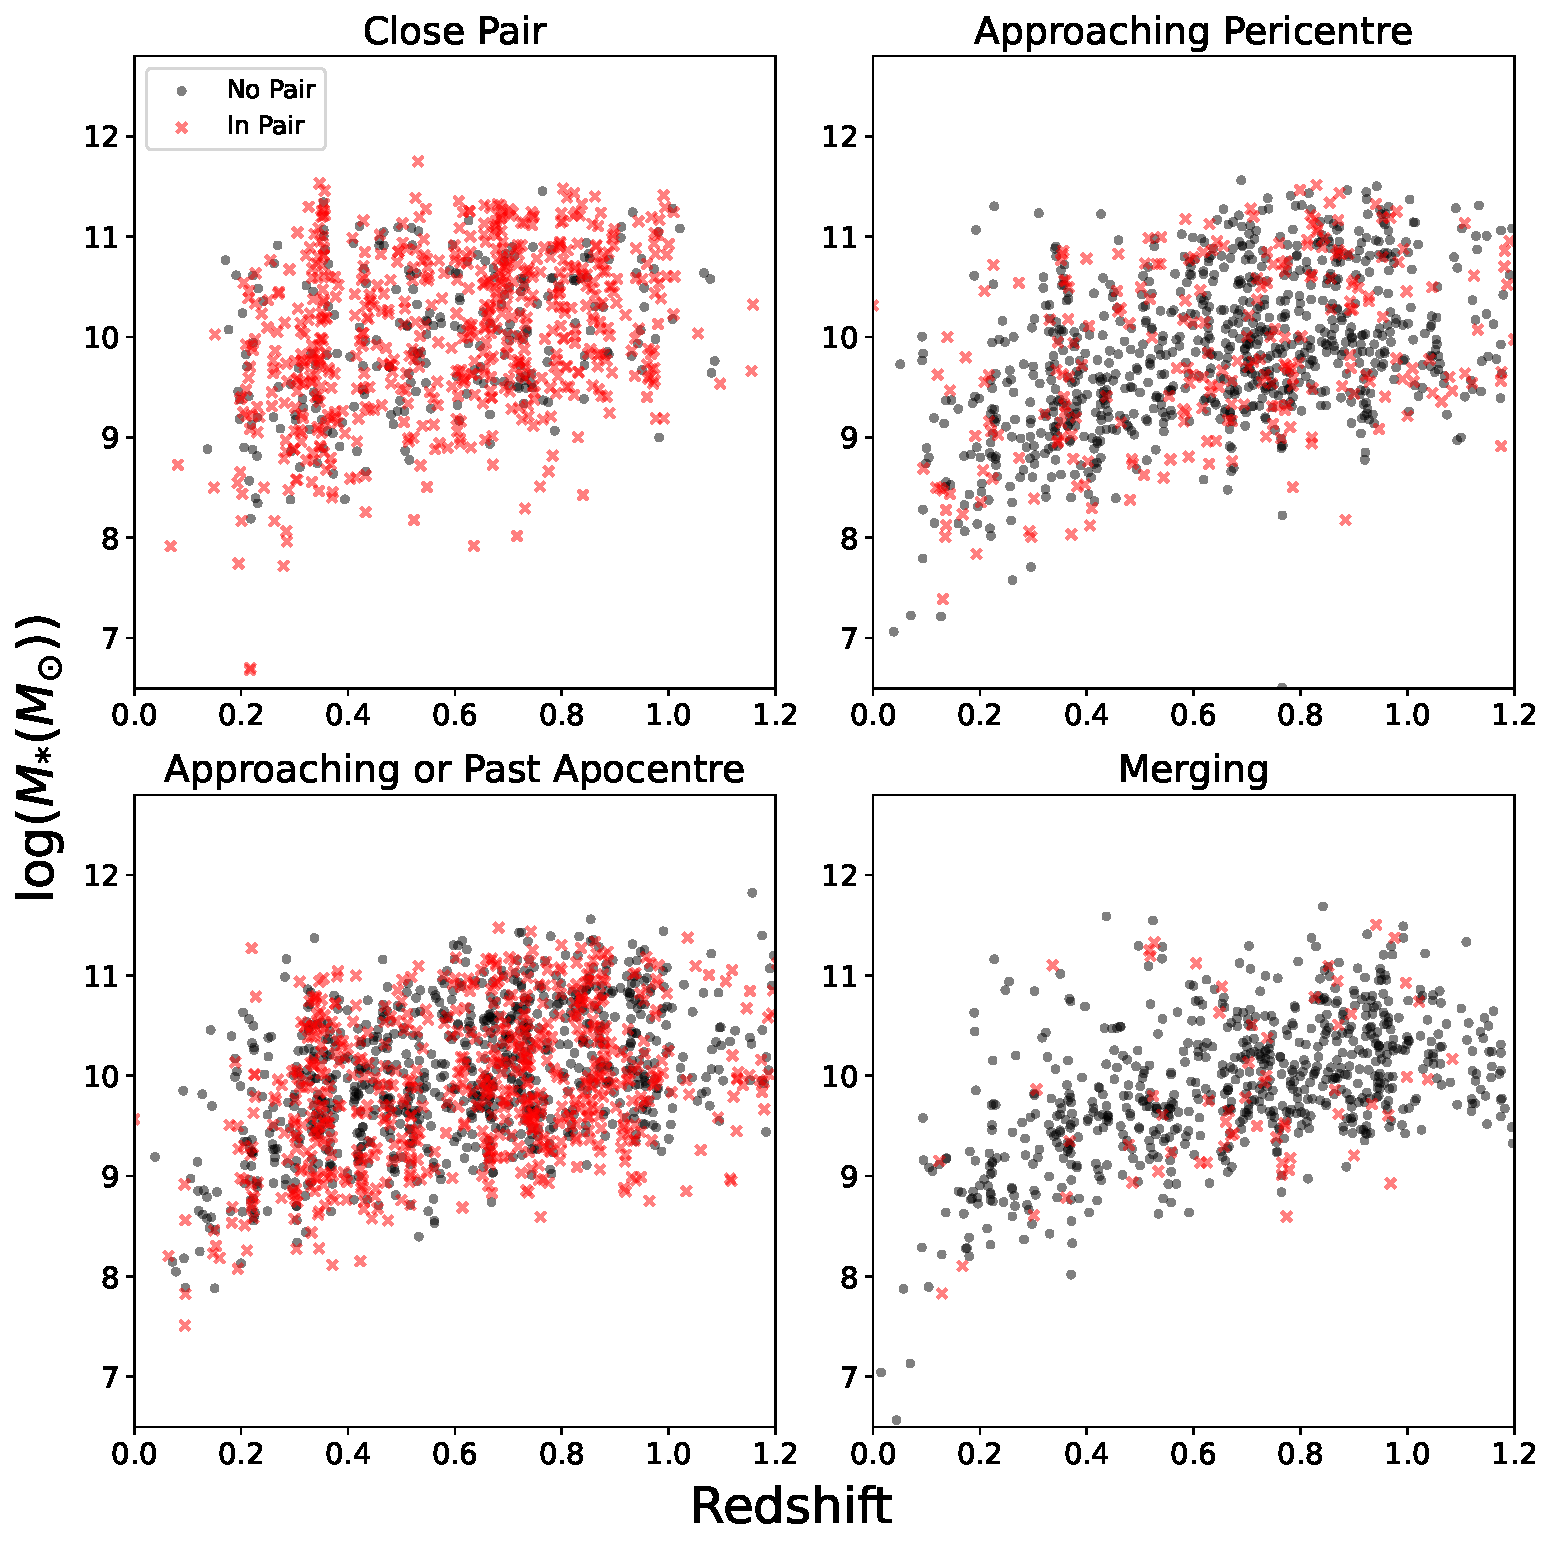
\includegraphics[width=\textwidth]{Chapter3/figures/redshift-limitations.pdf}
\caption[Redshift vs Mass distribution for each stage of interaction we have defined.]{Redshift vs Mass distribution for the four stages of interaction. We separate those systems with an identified secondary (in red) from those where no secondary could be found. The dashed blue line shows the mass cuts we make for our mass-limited sample and is set at $\log(\frac{M}{M_\odot}) \geq 9.25$. As shown here, the distribution of systems across redshift and mass is consistent for all stages in our sample. This is important as we use tidal distortion and the existence as tidal features as a fundamental for our classification methodology. Therefore, we are likely not affected by this in our analysis. We find that our ability to identify pairs is primarily affected by stage and not redshift.}
\label{fig:redshift_selection}
\end{figure}

Throughout this Chapter, we will use our mass-limited sample in our analysis. This gives us uniform sensitivity across our volume. However, we also conducted the same analysis described below with the flux-limited sample and the qualitative conclusions of this Chapter did not change.

\subsection{Sample Count Summary}\label{sec:sample-summary}
\noindent Thus, to briefly sumarise this chapter, we have applied multiple cuts and additions to our initial sample of interacting galaxies. We have gone from an initial sample of 3,689 matched galaxies with COSMOS to a mass-limited sample of 3,384 galaxies. This mass-limited sample of galaxies is the one we will use throughout this work. In the mass-limited paired sample there are 338 pairs or 676 galaxies.

\section{Method: Environment, AGN and Interaction Stage} \label{method}
A primary aim of this work is to investigate the evolution of different galactic parameters with stage of the interaction. Each stage is defined to capture a different part of the dynamical time and merger history. This stage also relates to the projected separation of galaxies with an identified secondary. Here, we define the short hand for the interaction stages and which part of the dynamical time they cover. We also describe how we find AGN in our full sample and find measurements of the environment about each. The parameters required to calculate the AGN fraction are not found in the COSMOS2020, and we therefore must cross match with other catalogues to find the required parameters. We also describe the catalogue we use to define the environmental density about each of our sources. This is important to consider, as it is well known that measured SFRs of galaxies can be affected by environment, as well as existing biases in where interacting and merging galaxies reside. We, therefore, need to check that we have not introduced any environmental biases into our definition of interaction stage. 

\subsection{Classifying Stage of Interaction}\label{sec:staging}
The primary goal of this work is to find if a relation exists between a host of galactic parameters, underlying physical processes and the stage of the interaction. Each stage covers a different part of the dynamical history in an interaction and, in this case, we define it based on the morphology and projected separation between systems. We have already encountered the four stages we will investigate in Figures \ref{fig:matched-distributions} and \ref{fig:redshift_selection} and now define a short hand name to refer to them as well as fully describe the part of the dynamical history they represent. These are:

\begin{itemize}
\item Separated: Systems which are well-separated with little to no morphological disturbance (Close pairs).
\item Pericentre: Close pairs showing morphological distortion while still in a pair or show a physical connection by tidal features.
\item Apocentre: Well separated pairs with morphological disturbance or isolated galaxies with clear tidal features.
\item Merging: Highly disturbed systems with a secondary core present.
\end{itemize}

\noindent Our four stage approach is not a new one, and many other works have utilised it to differentiate different parts of the dynamical history of a galaxy interaction \citep[e.g][]{2022ApJ...937...97C, 2023ApJ...952..122G}.

Figure \ref{fig:stages} shows the original source cutouts used in Chapter \ref{chapter2} to give an example of each stage. There are degeneracies associated with this staging system, however. In this context, we define a degeneracy as when the interacting galaxies may be at two or more parts of the dynamical timescale and we have no way to tell without further information on the system.

\begin{figure}
\centering
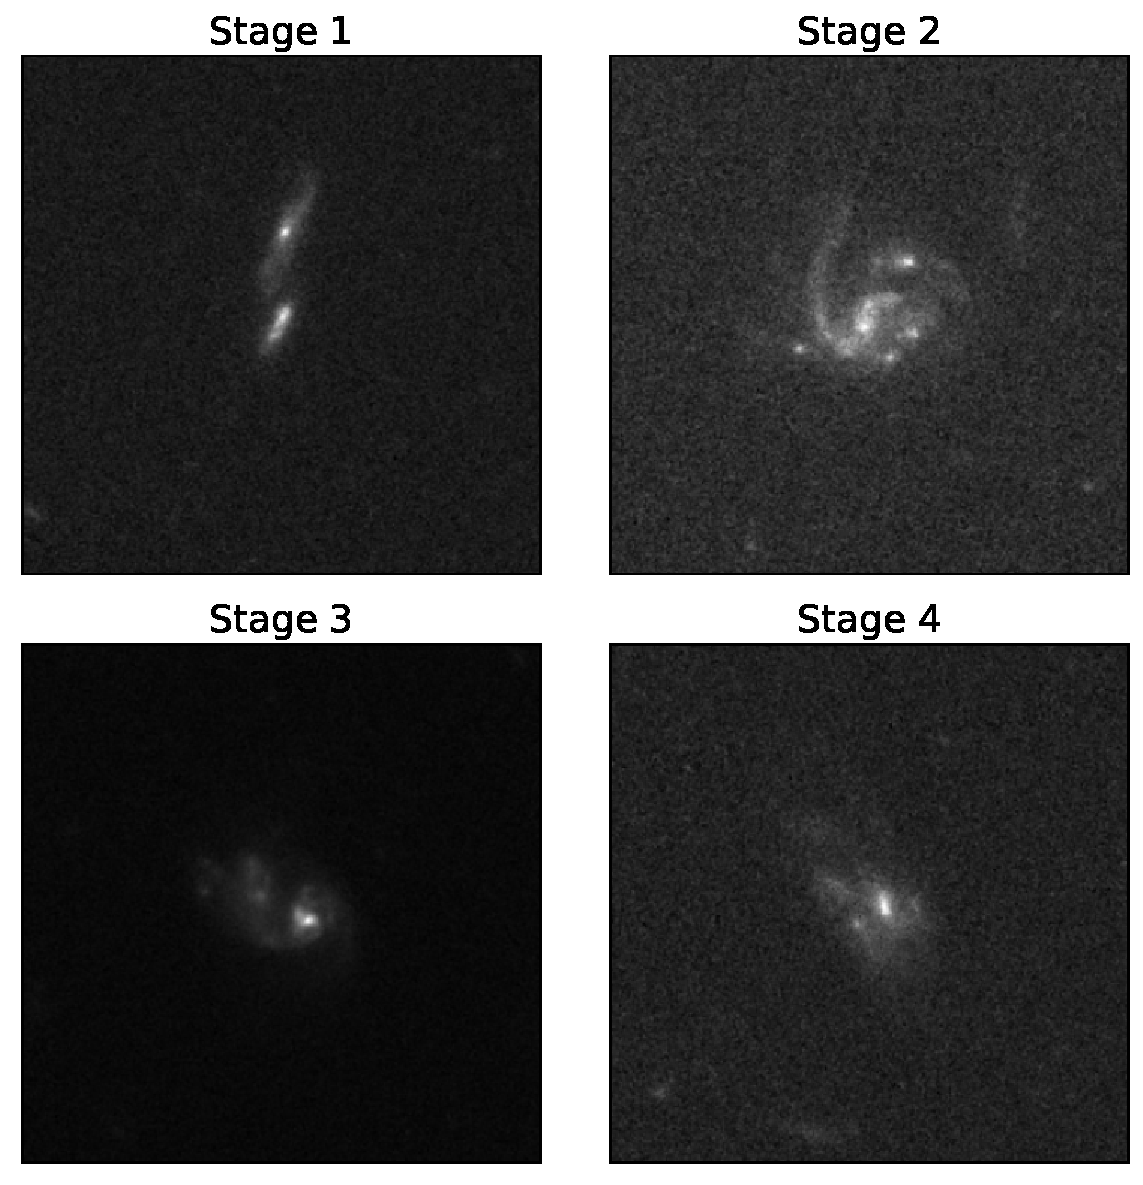
\includegraphics[width=\textwidth]{Chapter3/figures/examples-stages.pdf}
\caption[Examples of the four stages we split our interacting galaxy sample into.]{Examples of the four stages we split our interacting galaxy sample into. Separated: A close pair with confirmed redshift matching. Pericentre: Two distinct systems interacting with tidal features forming. Apocentre: A tidally disturbed system with no secondary present, likely at apocentre. Merging: A galaxy with multiple cores while highly disturbed. At the final stage before coalescence.}
\label{fig:stages}
\end{figure}

The separated stage of the interaction captures the first approach of the two systems and they are observed as a galactic pair. They have no morphological disturbance and, in our sample, are most often those galaxies with distinct disks. At this point, we would expect no change in the underlying processes of the galaxies from their control samples. Interaction has not taken place yet, and the two systems are morphologically intact. By definition, this stage requires an identified secondary galaxy and therefore has the highest number of identified secondaries with every system having a secondary that can be visually classified. This is also the least degenerate part of the dynamical time we are sampling due to a criteria of no morphological disturbance. Therefore, it is unlikely that the galaxies have already made a passage.

The pericentre stage of the interaction is defined as the point where the two galaxies in the interaction are at or just passing the pericentre of the tidal encounter. At this point, we find the beginning of morphological disturbance, the beginning of the formation of tidal features and some tidal debris. Due to the two systems having to overlap or connect via tidal features - by definition - this is the stge that suffers most from limited identification of the secondary galaxy. The COSMOS2020 catalogue often defines these two systems as a single system, and therefore, we lack information about their secondary. This stage is also highly degenerate in the context of the dynamical timescale of the interaction. Without further information, we are unable to define whether the galaxies involved at this stage are at the first, second, third, etc passage of the tidal encounter. We also do not know if they are approaching or have just passed pericentre.

The apocentre stage describes those interacting systems where the two disks are fully separated and distinct from one another. They have some morphological disturbance associated with them, but do not require a secondary galaxy to be put into this stage. If the galaxies have sufficient velocity they would escape from each other and, therefore, their secondary could be beyond our COSMOS2020 cutouts used to visually identify them. This is reflected in an even distribution of finding the primary and secondary in this stage. This stage also defines a large part of the dynamical timescale. It spans from separating from the secondary and after pericentre, to moving out to the apocentre of the interaction (or escaping with sufficient velocity), to falling back in towards the secondary galaxy again. Without velocity information, we have no way of finding if the galaxy is moving away or moving towards its secondary.

Finally, the merging stage represents the final step of a galaxy interaction. If the two galaxies do not have sufficient velocity to escape one another they coalesce and ultimately merge. We define this stage through the severe morphological disturbance of the galaxy involved as well as the existence of a second core within it. While we attempt to capture only pre- or ongoing-coalescing systems, it is important to note that this stage is degenerate to post-merger remnants which will also be accepted by our criteria. Post-merger remnants are systems where coalescence has been completed and immediately after will be highly morphologically disturbed and difficult to distinguish from those systems with merging ongoing. At this stage, we would expect the interaction will be at its most violent with complete disruption of both galactic disks and likely increased star formation across the galaxy. 

We have noted the degeneracy of each stage as we have described them. Thus, we can now put this fully into the context of the dynamical timescale. Over a typical interaction, we would expect the galaxy pair to move from being separated to the pericentre of the interaction in the early times of the dynamical timescale. Then, dependent on the velocity of the system, the galaxy pair will either move straight into the merging stage of classification and begin to coalesce or it will move towards the apocentre stage. This change from pericentre to apocentre can then take two branching paths dependent on the velocity in the system. If the galaxies have sufficient velocity, the apocentre stage will be their end state until the tidal features slowly dissipate. If they do not have enough velocity to escape on another, the system will move from the apocentre stage back into the pericentre stage. This could then happen for many cycles until finally the galaxies enter the merging stage and coalesce. Figure \ref{fig:illustration} shows the branching paths that the galaxies can take through each stage. These images are created using the Advanced Python Stellar Animation Module restricted numerical simulation, described in Chapter \ref{chapter4}, and are for illustrative purposes only here.

\begin{figure*}
\centering
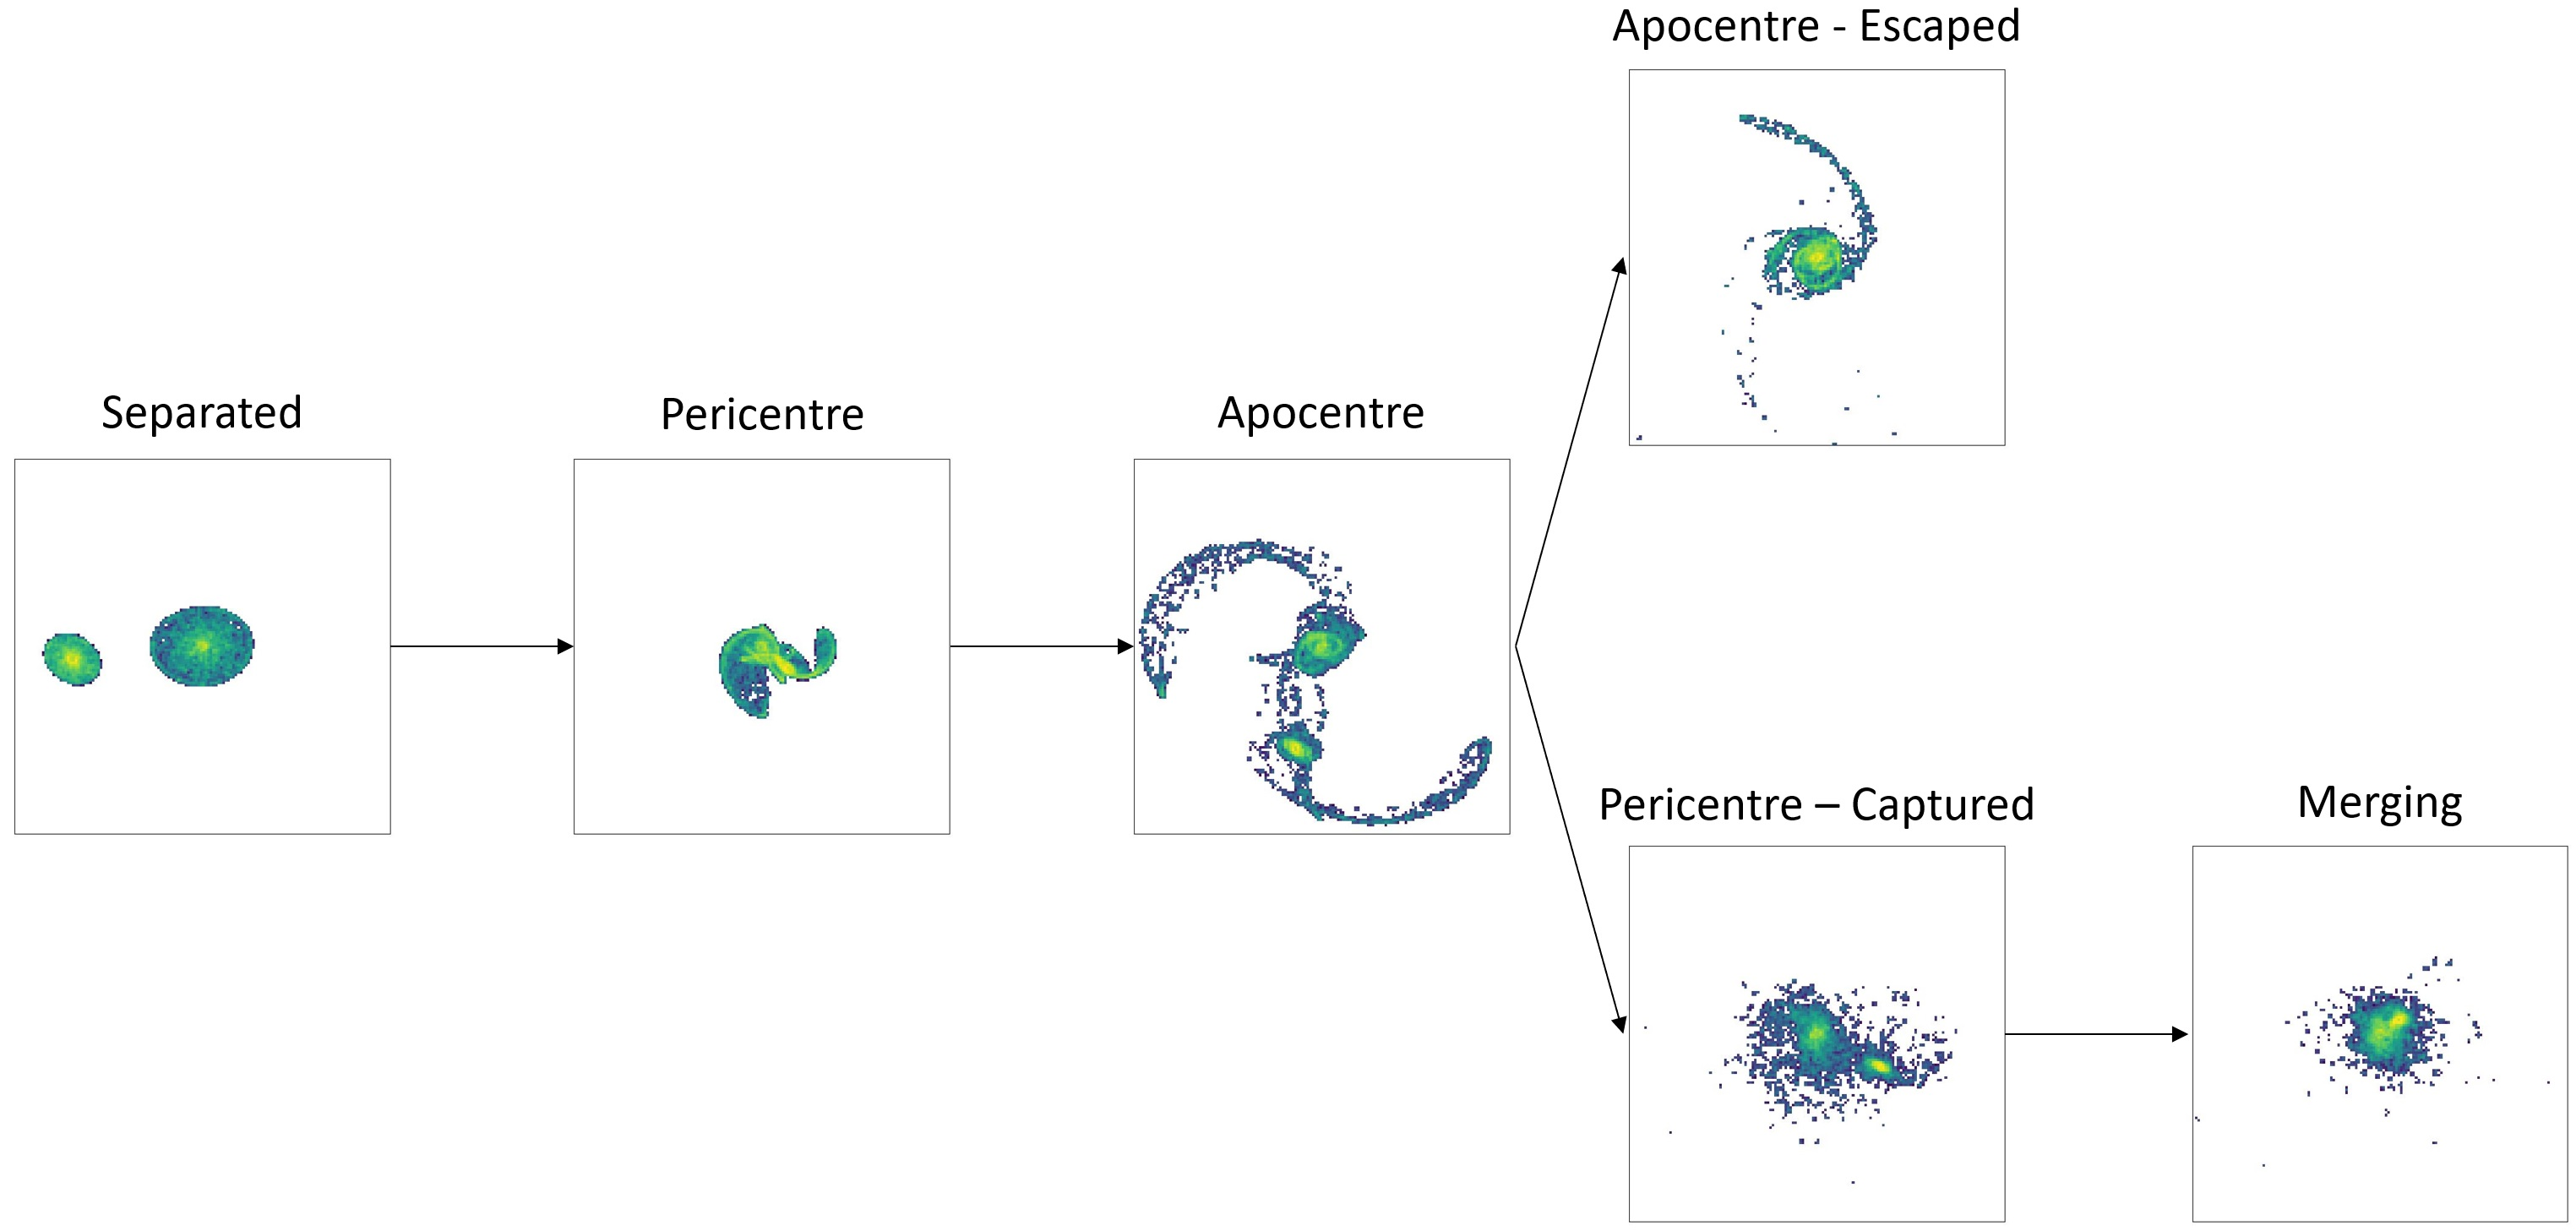
\includegraphics[width=\textwidth]{Chapter3/figures/stage-evolution.jpg}
\caption[The progression through an interaction using our stage definitions.]{The progression through an interaction using our stage definitions. In the separated stage, we have two systems that are approaching each other but exhibit no tidal features. This is before the point of closest approach has occurred. This is followed by an intial pericentre stage: the systems are approximately at their closest approach. This stage is often mistaken, in the COSMOS catalogue, for being of only one source. Clear tidal features exist with major disturbance in the two disks. This is followed by the apocentre stage, where there are two distinct cores with clear tidal features. However, after this point, there are two outcomes to the system depending on the galactic velocities. If the secondary has the escape velocity, the system will remain an apocentre stage interaction until the tidal features dissipate (and no longer are in our sample). If they do not have enough energy, the system will return to the pericentre stage of the encounter and then begin to coalesce in the merging stage. Images are from the Advanced Python Stellar Particle Animation Module interacting galaxy algorithm described in Chapter \ref{chapter4} and based on the stellar particle animation module algorithm described in \citet{2016A&C....16...26W}.}
\label{fig:illustration}
\end{figure*}

As described previously, in the literature, rather than using the stage of an interaction based on morphology the projected separation of the two systems is used. To explore the difference between using our staging system and the projected separation, as well as to ensure we recover the expected relations, we measure the projected separations of our confirmed galaxy pairs. Figure \ref{fig:proj-seps} shows the stage classification with projected separation between the two pairs. We measure this by taking the average of the best fit photometric redshifts between the two galaxies, and converting their angular separation to a physical one. The most distinct projected separation ($s_{\mathrm{proj}}$) in stages is between the pericentre and apocentre stages. Here, we see that the percentre stage is dominated by systems with $s_{\mathrm{proj}}<$35kpc while the apocentre stage is dominated $25 \leq s_{\mathrm{proj}} \leq 100$ kpc. The pericentre stage is visually classified as systems which are highly morphologically disturbed, while either being morphologically linked to each other or overlapping. Those galaxy pairs with large projected separations are pairs which are very large in angular size, while still overlapping or morphologically linked. If this criteria is not met, then the system becomes an apocentre stage interaction where the two galaxies in the pair are completely distinct. There is some overlap between the projected separations of the pericentre and apocentre stage as this is somewhat dependent on the angular size of the two systems involved in the interaction.

\begin{figure*}
\centering
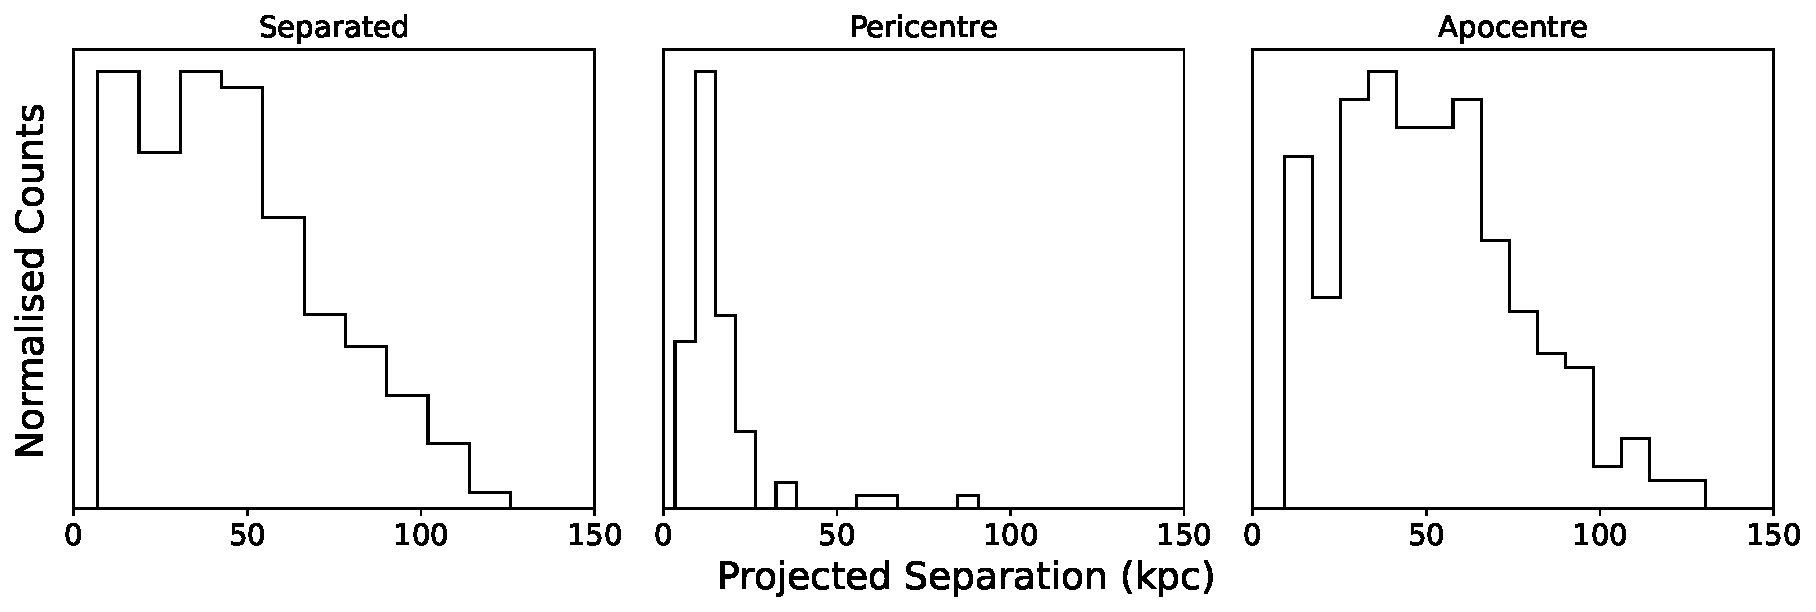
\includegraphics[width=\textwidth]{Chapter3/figures/projected-seps.pdf}
\caption[The projected separations of the confirmed galaxy pairs in our sample.]{The projected separations of the confirmed galaxy pairs in our sample. This confers with other works the definition of our different stages. The separated stage can be at any projected separation, however, we have visually confirmed that these sources are not morphologically disturbed. The pericentre stage is dominated by systems with small projected separation as, by definition, they must be morphologically linked or overlapping. Those systems at larger separation are very large systems whose morphology categorise them as at the pericentre stage. Finally, apocentre stage galaxies are those which are visually confirmed to be fully morphologically separated and tidally disturbed. The bulk of these lie in a range of 25 - 100kpc in projected separation from each other. There is some overlap between the pericentre and apocentre stages in projected separation, as their visual classification is also dependent on the system size.}
\label{fig:proj-seps}
\end{figure*}

Figure \ref{fig:proj-seps-limits} shows the overlap between our four stages in projected separation. It also shows the limitations in our sample of finding the secondary galaxy in the interaction. This, primarily, is at low redshift where a larger projected separation represents a larger angular separation on the sky. This is a limitation of using visual confirmation of the secondary within a cutout of limited angular size. Thus, we see at low redshift ($z < 0.2$) we only identify pairs of galaxies with projected separation below $50kpc$. Towards our limiting redshift, however, we are able to identify galaxy pairs down to a projected separation of 10kpc, as well as out to 200kpc. 

% Need to integrate this figure.
\begin{figure*}
\centering
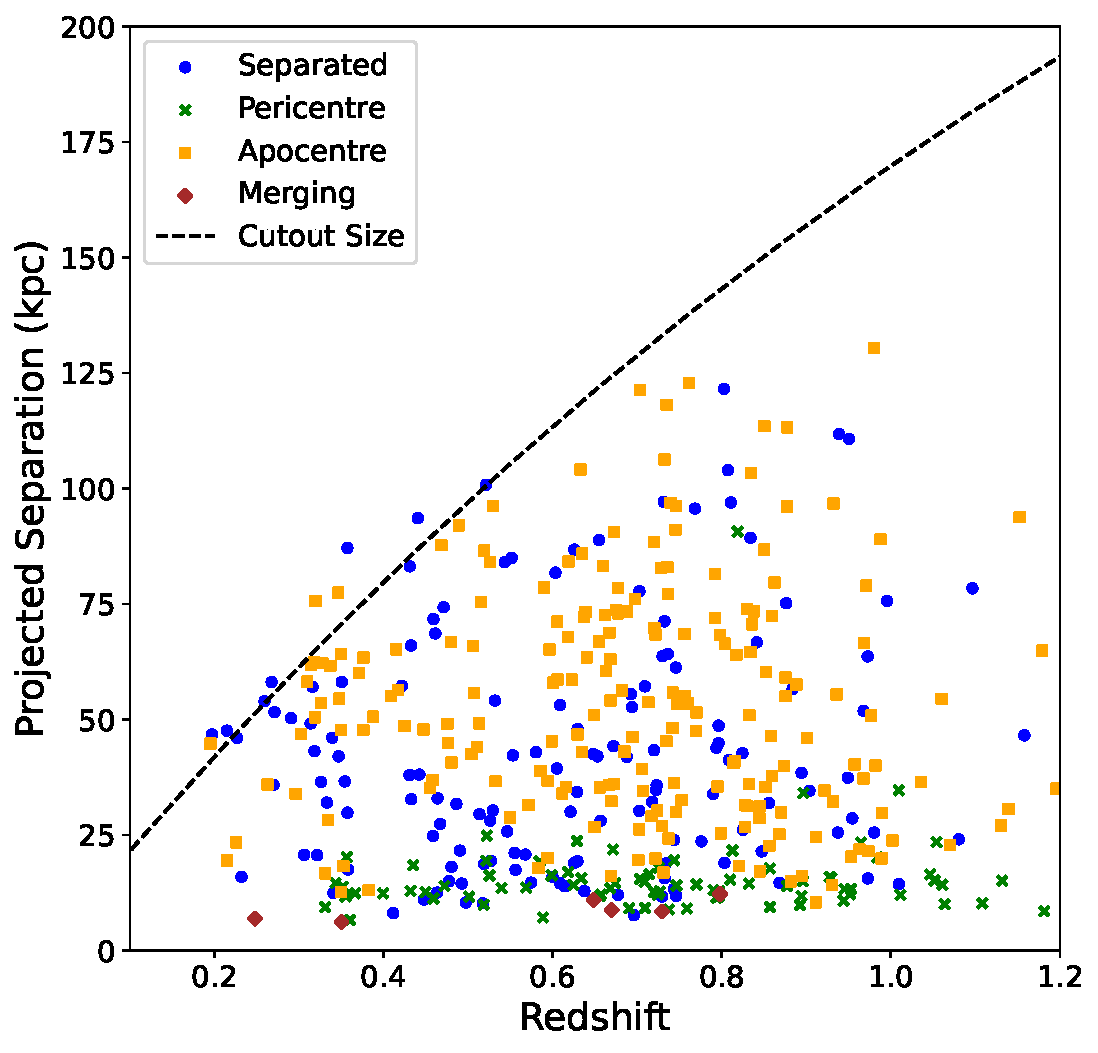
\includegraphics[width=\textwidth]{Chapter3/figures/redshift-proj-sep-diagnostic.pdf}
\caption[The measured distribution of projected separation with redshift.]{The measured distribution of projected separation with redshift. As we have made redshift cuts out to $z = 1.2$, we investigate the limitations on the projected separations we can successfully identify across our volume. We find that we can successfully identify secondary galaxies and their projected separations down to 10kpc to $z=1.2$. This is true across defined interaction stage. We find, because of the defined size of our cutouts, the limitation of finding the secondary galaxy is at low redshift.}
\label{fig:proj-seps-limits}
\end{figure*}

We will use the projected separation to investigate relations between AGN activity and if we observe enhancement in star formation. The SFR is already present in the COSMOS2020 catalogue as measured using \texttt{EAzY}/\texttt{FAST}. To ensure that any enhancements are from interaction alone, we must ensure we have no biases in the environment distribution of our sample. First, we describe how we classify the environment of each of our matches.

\subsection{Matching to Environment Catalogue}\label{data:environ}
\noindent It is well known that the environment has a direct impact on the observed SFR of galaxies. A galaxy in a cluster environment has, on average, a higher SFR than those in the field \citep{2006MNRAS.373..469B}. Thus, if any of our stage classifications are biased towards one environment or another, it could impact our results.

There is no measure of the environmental density in the COSMOS2020 catalogue. Such a measure is often calculated in numerous ways, such as the N-nearest neighbour \citep{2006MNRAS.373..469B}, different Bayesian metrics \citep{2008ApJ...674L..13C} or estimating it from Voronoi Tesselation \citep{2021inas.book...57V}. However, in this Chapter, we use the existing environmental density catalogue produced by \citet{2017ApJ...837...16D}. This catalogue was created specifically for the COSMOS survey, and has a measured density for all sources with mass $\log(\frac{M}{M_\odot}) \geq 9.6$ and $z \leq 1.2$. \citet{2017ApJ...837...16D} calculate not only the density, but also the density parameter $\delta$ and assign each source to a field, filament or cluster classification. For a full description of how they calculate the environment and density field see \citet{2015ApJ...805..121D} and \citet{2017ApJ...837...16D}, but we will briefly describe it here.

To build the density field throughout the COSMOS field, \citet{2017ApJ...837...16D} first construct a set of overlapping redshift slices. Within each slice, a subset of the galaxies are selected such that the median of the probability distribution function (PDF) of their photometric redshift is within it. Then, from this subset, they calculate the weighted surface density within the redshift slice. The weighting is based upon the PDF of the photometric redshift present within the redshift slice. These weights significantly reduce the effects of projection effects. They then apply a weighted adaptive kernel smoothing using a 2D Gaussian kernel whose width changes based on the found local density of galaxies. Once this density field is created, the density around the sample galaxies can simply be interpolated across the density field based on the angular position and the redshift slice the sample galaxy is in (based on its photometric redshift PDF).

The result of this process, and the cuts defined previously, is a catalogue of $\approx$45,000 galaxies with their densities accurately measured. We remove any sources which are flagged as uncertain from the catalogue (a flag in it) providing us with $\approx$39,000 sources with which to cross match the sample from Chapter \ref{chapter2}. We apply the same cuts to our sample as applied in \citet{2017ApJ...837...16D}, and only consider those systems with a mass $\log(\frac{M}{M_\odot}) \geq 9.6$. To cross match with our sample, we use the COSMOS2015\_ID which exists in both the COSMOS2020 catalogue and the \citet{2017ApJ...837...16D} catalogue. Upon applying the mass cut to our sample, we find 2,800 matches to the \citet{2017ApJ...837...16D} catalogue. Upon matching based upon the COSMOS2015 ID, we find that 628 sources in our sample do not exist in the environment catalogue. This reduces our sample to 2,172 galaxies with confirmed and reliable environment density measurements.

\subsection{Classifying AGN}\label{sec:agn-clsf}
\noindent We will also investigate the effect of interaction stage on AGN activity throughout our sample. As the COSMOS2020 catalogue does not contain the relevant parameters to make this calculation, we turn to the Chandra COSMOS Legacy Survey Multiwavelength Catalogue \citep{2016ApJ...817...34M} and the COSMOS VLA 3GHz survey \citep{2017A&A...602A...6S, 2017A&A...602A...3D}. Both of these catalogues span the entire COSMOS area, and contain detailed classifications of the sources they find. The Chandra survey spans the X-ray range of wavelengths, and successfully identified numerous X-ray AGN. The VLA 3GHz survey is a radio survey, and we use this to find the radio AGN through our sample. 

Our matching process is similar to previously described matching processes. We use the previously identified COSMOS2020 source coordinates and select the nearest source with in a 10" matching radius. We first find matches of radio AGN using the VLA 3GHz survey catalogue and then search the Chandra survey. At every step, if we find a match in the relevant catalogue, we remove it from subsequent searches in other catalogues and take the first classification as the correct one.

Applying our matching criteria, we find 1,059 matches in the VLA 3GHz survey and 155 in the Chandra survey. From existing flags within the catalogues, these were split into 812 star forming galaxies and 402 AGN. We also investigate cross matching with the MPA-JHU catalogue \citep{2003MNRAS.341...33K, 2004MNRAS.351.1151B, 2007ApJS..173..267S}, however, found that all matches were already represented by the VLA and Chandra surveys. We also use the COSMOS XMM-survey and, again, find no new sources to add to our sample. While the ratio of AGN to star forming galaxies in our sample seems large compared to other works, it is important to note that this is a result of limited matching between the catalogues. Of the 4,181 galaxies in our sample, only 1,214 appeared at all in either the VLA or Chandra catalogues.

\subsection{Visual Classification: Sources of Contamination}
\noindent Throughout the description of our sample, we have identified these interacting systems by a combination of visual classification and the best-fit photometric measurements from the COSMOS2020 catalogue. This introduces limitations which could bias or contaminate our sample. We identify three serious areas of bias or contamination: 1) error inherent from using only photometric redshift measurements, 2) failure of identification of tidal features at higher redshifts due to surface brightness dimming and reduction in angular size, and 3) mis-identification of tidal features as disturbances caused by other processes. In this subsection, we will address each of these points and quantify how they affect our sample. We will also discuss any how we mitigate these effects where appropriate.

First, there is always an inherent error in using the photometric redshift measurements of galaxies. We briefly mentioned this when describing pericentre stage systems. There, we found $\sim50$ systems which were clearly morphologically disturbed with linking tidal features, but their photometric redshifts were such that they couldn't possibly be interacting. It is also possible that we have missed pair identifications in the separated stage (where no tidal features are expected) due to incorrect photometric redshifts. We wish to quantify both these effects. \citet{2022ApJS..258...11W} quantify the error in their photometric redshift calculations (which we use here) as $<1$\% for our redshift and flux range. They quantify the scatter in the distribution of photometric to spectroscopic redshifts is $0.025(1+z)$ within our redshift and flux range. This leads to a maximum error on our photometric redshifts in this range of $\pm0.06$. 

\begin{figure}s
\centering
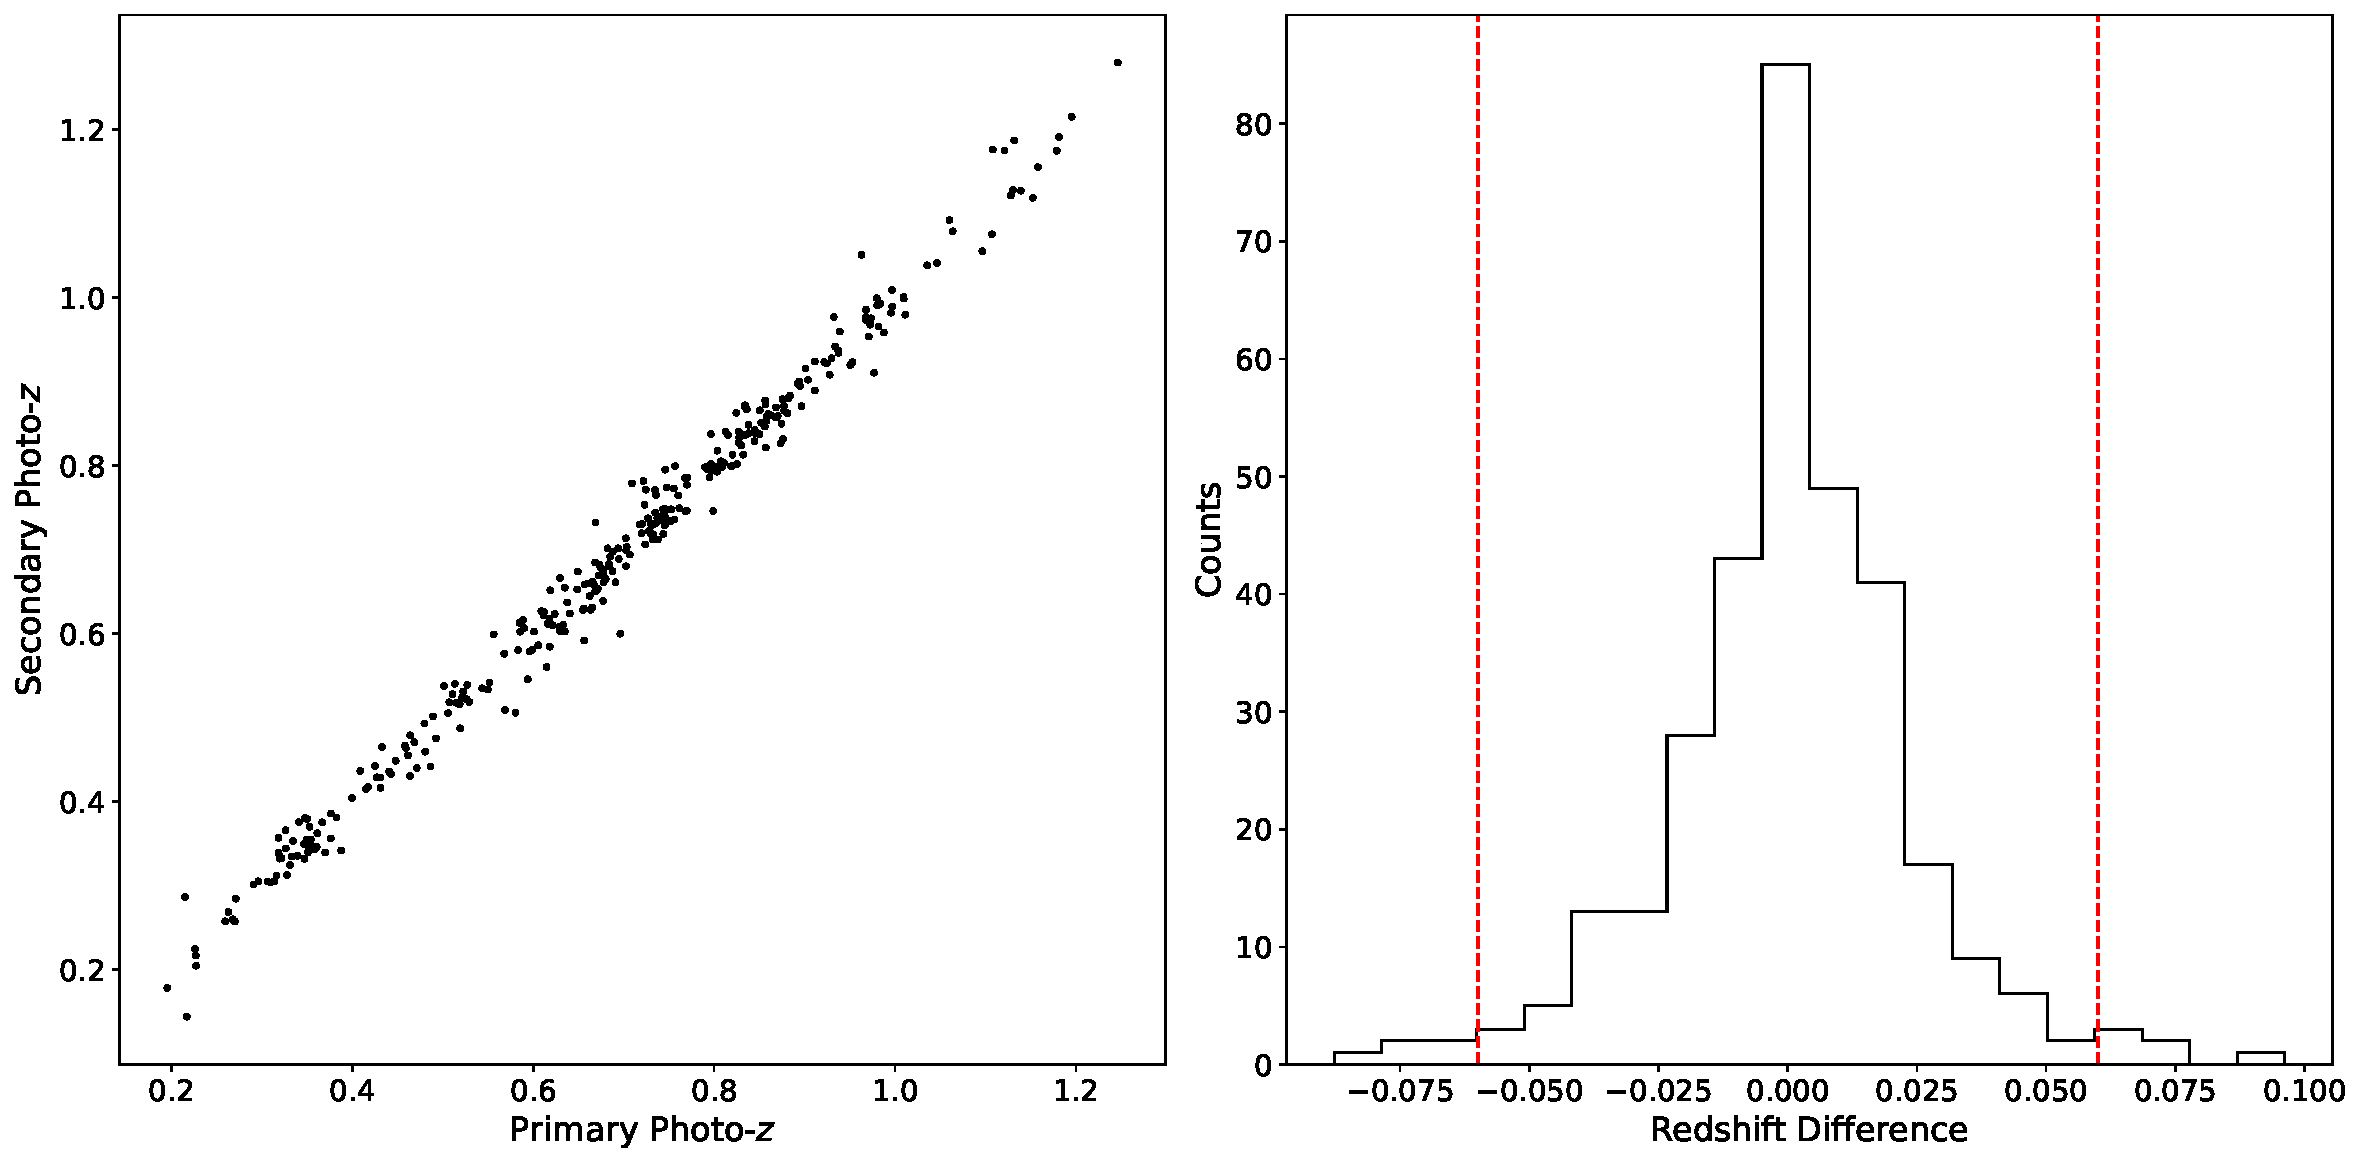
\includegraphics[width=\textwidth]{Chapter3/figures/redshift_scatter.pdf}
\caption[The scatter in photometric redshifts of our paired sample.]{The scatter in photometric redshifts of our paired sample. Left shows the scatter in the primary and secondary photometric redshift measurements. Right the measured difference in the primary and secondary photometric redshifts found in the left panel. The red dashed lines show the expected error at the maximum redshift of our sample. As shown, the bulk of the sample lies within this region.}
\label{fig:redshift-scatter}
\end{figure}

To investigate the affected systems, we therefore look at the redshift distribution of our paired sample. Figure \ref{fig:redshift-scatter} shows the scatter in our found pairs as well as the difference between them from our visual classification. During the visual classification, we instituted a cut that each interacting pair must be within a photometric redshift difference of $\pm0.1$. To estimate our completeness, we apply a bootstrapping test to our sample and see the number of systems we may have removed from our sample with this cut. We create a simulated paired sample of 10,000 systems and apply an error measurement based on the photometric redshift errors. This gives a paired sample across our redshift sample at slightly different redshifts. We then apply our cut, and check how many systems we would remove due to the photometric error from the COSMOS2020 catalogue. We find that we would retain $\approx91$\% of the sample with this cut, given the photometric redshift error. This is a lower limit on what we have retained, as we have not considered possible tidal features that would have caused us to keep the system in our sample. Therefore, we are unlikely to have removed a large percentage of interacting galaxies due to the photometric redshift error and the cuts we have applied.

The resultant scatter in photometric redshifts between the primary and secondary in our paired sample is shown on the left panel of Figure \ref{fig:redshift-scatter}. The right hand panel shows the distribution of the difference measured between the primary and secondary photo-$z$s, with the red dashed lines showing the maximum expected error on the photometric redshift measurement at the highest redshift of our sample. As shown, the bulk of our paired sample lies at very low redshift difference, meaning we are unlikely to have removed too many systems. This leads us to conclude that our pair selection process has been robust.

The second limitation of our approach is the failure of identifying interacting systems at high redshift due to missing the tidal features of the system. This would be a combined result of the affects of surface brightness dimming of their disks and tidal features at high redshift and while also having a small angular size. The former issue is mitigated by our limiting of our sample to be within a range of $0 \leq z \leq 1.2$ and with our mass limit of $9.25 \leq \log \frac{M}{M_\odot} \leq 12.5$. The latter is more difficult as we have a standardised cutout size which does not depend the redshift, or angular size of the system. This means that if a system were at redshift 1.2, our pixel resolution corresponds to roughly $0.5\rm{kpc~pix}^{-1}$ limiting the tidal features we would be able to identify. With such a scale we are able to identify extended tidal features away from the galactic disk such as tidal arms, but lack the resolution to those features which would be much closer to the disk. Thus, those interacting systems which have formed features such as shells, small tidal bridges or stellar streams will be missing from our samples at higher redshifts. Thus, at high redshift, we are most sensitive to the separated, apocentre and merging stage interacting systems while lacking the required resolution to pickup more intermediate tidal features at the pericentre stage.

To investigate how we are affected by this, we look at the change in found fraction of micro, minor and major interactions across our redshift range. The effect of surface brightness dimming will be related to the type of interaction we are observing, and the resultant flux distribution of the tidal features. To get an idea of this, we split out pair sample into its constituent interaction types based on the mass ratio. We define the mass ratio such that the primary galaxy contains the highest stellar mass in the pair. If there is more than two galaxies involved in the interaction, we take the primary galaxy to be the galaxy with the highest stellar mass in the system. We define three different interaction types based on the mass ratio: micro (where the mass ratio is less than 1:10), minor (where the mass ratio is between 1:10 and 1:3) and major (where the mass ratio is greater than 1:3). We would expect that major interactions would not be changed by surface brightness dimming across redshift as these interactions create strong tidal features. Micro interactions, on the other hand, will likely be highly affected by surface brightness dimming. Micro interactions are such that the secondary is often completely destroyed in the interaction, leaving stellar streams about the primary galaxy. These tidal features will be in the low surface brightness regime, where they will quickly be lost at high redshift.

\begin{figure}
\centering
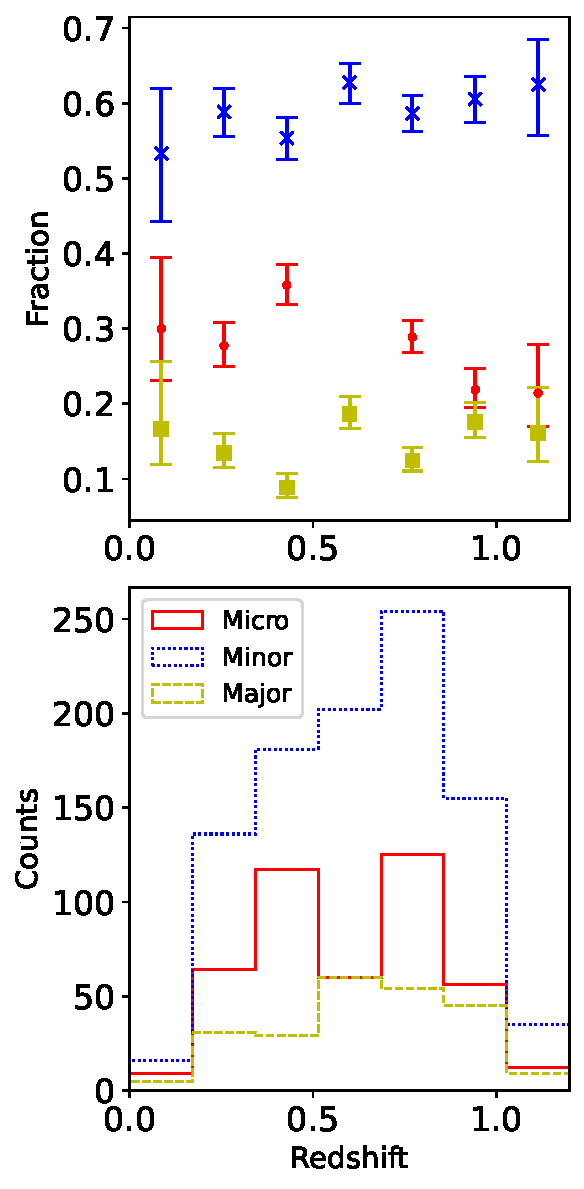
\includegraphics[width=0.55\textwidth]{Chapter3/figures/mass-ratio-limitation.pdf}
\caption[The change in found interaction type across our redshift distribution.]{The change in found interaction type across our redshift distribution. We define interaction types from the mass ratio of paired galaxies in our paired sample. \textit{Bottom}: The distrition of different interaction types across redshift. \textit{Top}: The change in the fraction found of different interaction types with redshift. As expected, the minor and major interaction fractions remain consistent with redshift but the micro interaction fraction declines. This is a result of surface brightness dimming on the tidal features formed in the interactions. In a micro interaction, we would see the complete destruction of the secondary into stellar streams about the primary galaxy. Such a tidal feature would be in the low surface brightness regime, and quickly be lost at increasing redshift. However, the change in fraction we find across our redshift range is not high enough to alter our conclusions.}
\label{fig:mass-ratio-limitation}
\end{figure}

Figure \ref{fig:mass-ratio-limitation} shows the distribution of interaction types across redshift. The bottom panel shows the distribution in galaxy counts across redshift for the mass-limited sample. The top panel shows the change in the fraction of each interaction type we find in each redshift bin. For the minor and major interactions, we see that there is little change in the fractions across our redshift distribution. However, as expected, with micro interactions we see a gradual decline in the found fraction with increasing redshift. This shows a loss in sensitivity to this interaction type but over our redshift distribution there is not significant change that could change our conclusions. Therefore, we show this as a warning to those who might use our methodology over a wider redshift distribution.

The final limitation of our approach we discuss is of relying on visual classification to identify interacting galaxies. Besides the issue of close pairs (described in previous sections) there is also assuming the disturbance of the systems is due to interaction, and not from other processes. The most obvious process which could mimic tidal disturbance is that of ram pressure stripping (RPS). RPS is an effect of the galactic environment stripping out the gas within a galaxy, and causing the formation of what appears like debris about the galactic disk. It can also cause major disturbance and irregular morphology. Thus, this could easily be a form of high contamination in the apocentre and merging stages of our sample. The environment that RPS is most prevalent is that of a cluster environment. Therefore, if we are highly contaminated to identifying RPS galaxies as interacting galaxies, we would see a bias in the environment of our sample towards galaxy clusters. To check this, we measure the distributions of our galaxies in each environment with stellar mass. We use the sample matched to \citet{2017ApJ...837...16D} as described in Chapter \ref{data:environ}.

Figure \ref{fig:dens-stage} shows the distribution of our matched samples with their density values with Figure \ref{fig:environ-fract} showing the change in environment fraction with stage. It is important to note that \citet{2017ApJ...837...16D} has a higher mass cutoff than we have implemented in our underlying sample. Therefore, this is showing the density of all systems $\log$M$_*$/ M$_\odot \geq$ 9.6. We conduct weighted Kolmogorov-Smirnov \citep[KS-test;][]{an1933sulla} and Anderson-Darling \citep[AD-test;][]{stephens_74} on the environment distributions. The KS-test is excellent at comparing different weighted distributions and indicating if they are drawn from the same parent sample. The AD test tests for this similarity as well, and we use both to ensure consistency and robustness in our measurements. These tests confirm they are likely drawn from the same parent sample, with the resultant $p$-values $\approx1$ the distributions. Thus, we can confidently state there are no biases in our stage selection with environment, and it fair to assume that any evolution we find between interaction stages is due to interaction and not due to biases in the environment of our stages samples.

\begin{figure}
\centering
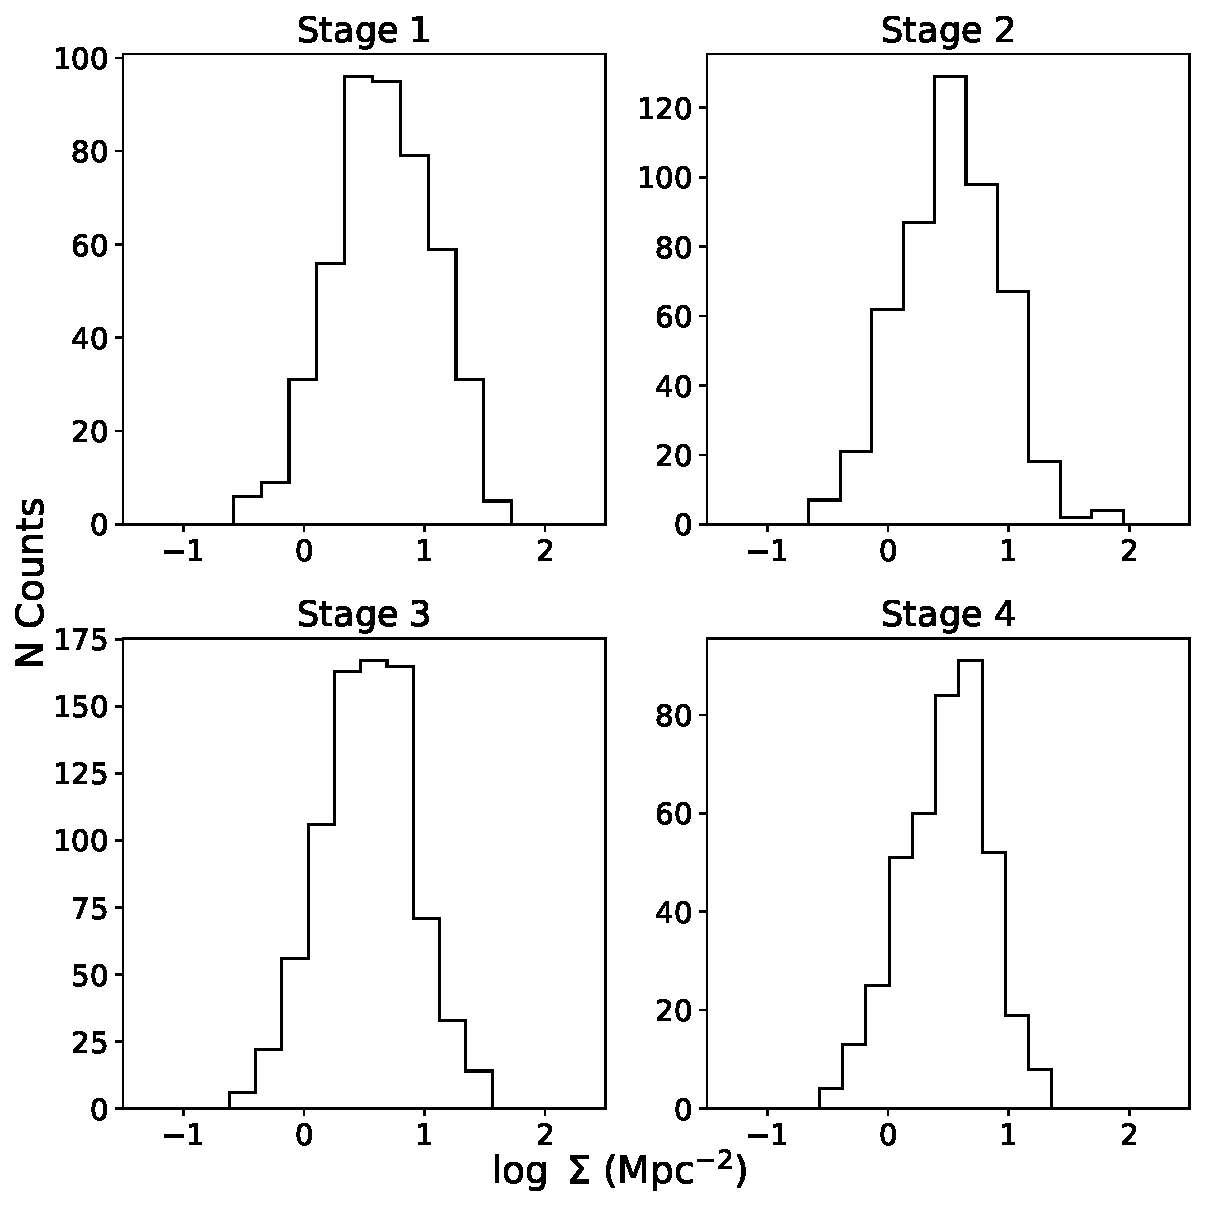
\includegraphics[width=\textwidth]{Chapter3/figures/density-stage.pdf}
\caption[The density about each of our sources matched with the \citet{2017ApJ...837...16D} catalogue.]{The density about each of our sources matched with the \citet{2017ApJ...837...16D} catalogue. As shown, there is no existing bias in the distribution of galactic environments throughout our stages. Therefore, that we have identified primarily tidal affects and not environmental ones.}
\label{fig:dens-stage}
\end{figure}

\begin{figure}
\centering
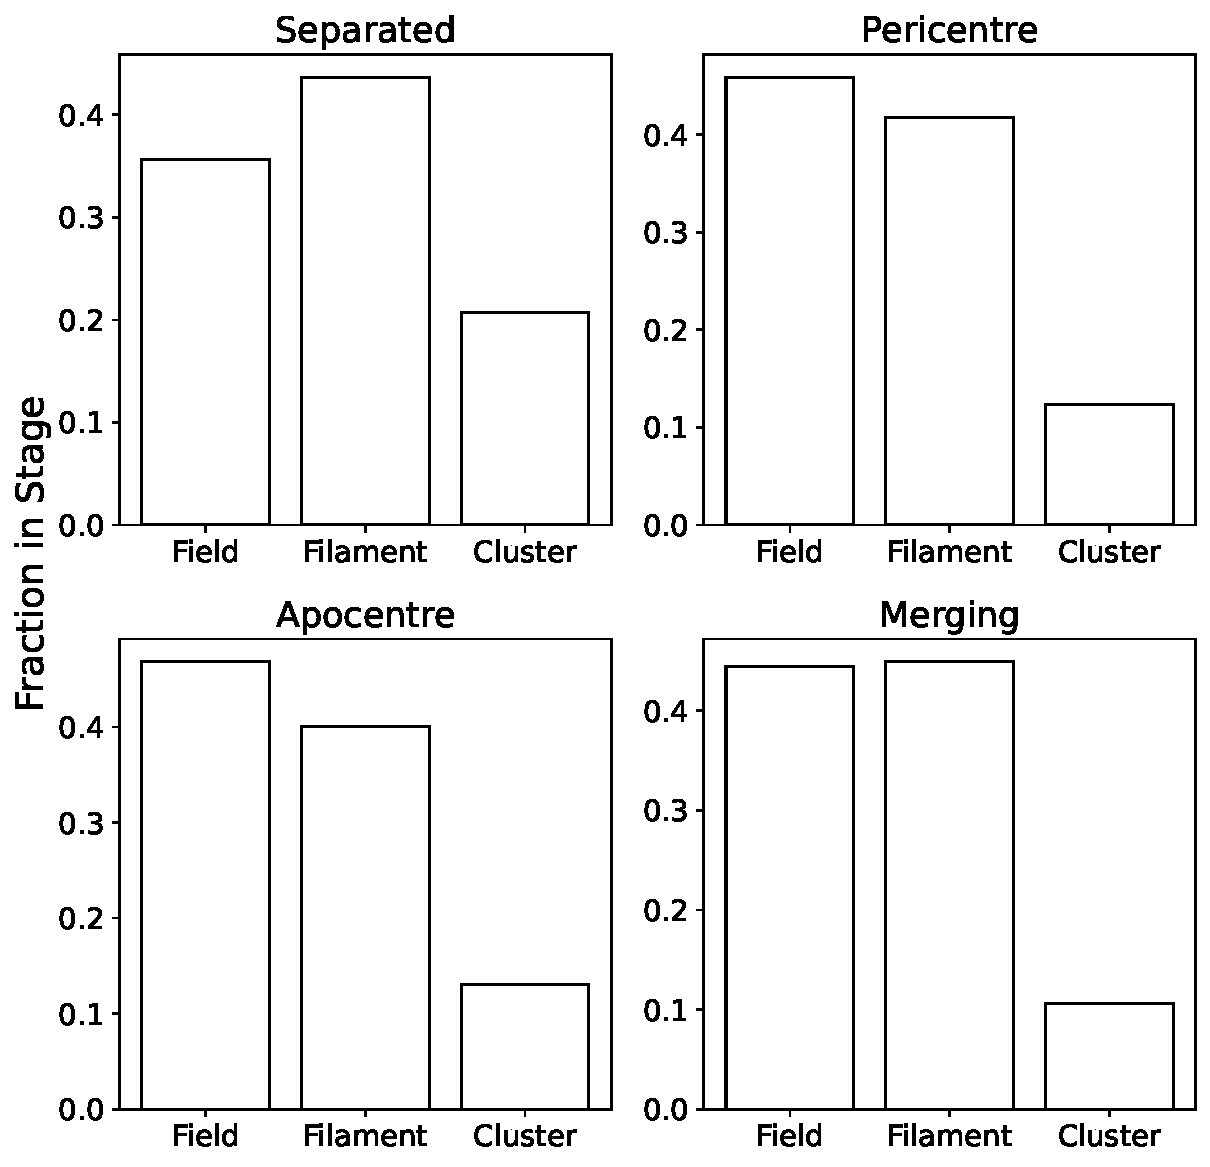
\includegraphics[width=\textwidth]{Chapter3/figures/environment-fractions.pdf}
\caption[The fraction of galaxies in each stage in different environments.]{The fraction of galaxies in each stage in different environments. This reinforces that there is no overarching bias between our samples for the cluster environment. In the cluster environment, RPS could lead to morphologies which appeared like tidal disturbance.}
\label{fig:environ-fract}
\end{figure}

To reinforce this, Figure \ref{fig:dens-sfr-mass} shows the environment classification in our reduced stellar mass-SFR distribution. This shows that there is no ordered structure, or bias, in our sample with environment and further reinforces that the galactic environment is not responsible for effects we may find from interaction. The majority of our sample lie either within filaments or in the field. The environment which would have the most effect upon the SFRs of our sample is a cluster environment. However, the fraction of our sample within a cluster is never greater than $\sim20$\%. Therefore, the lack of information here does not have a large impact on this measurement. 

\begin{figure}
\centering
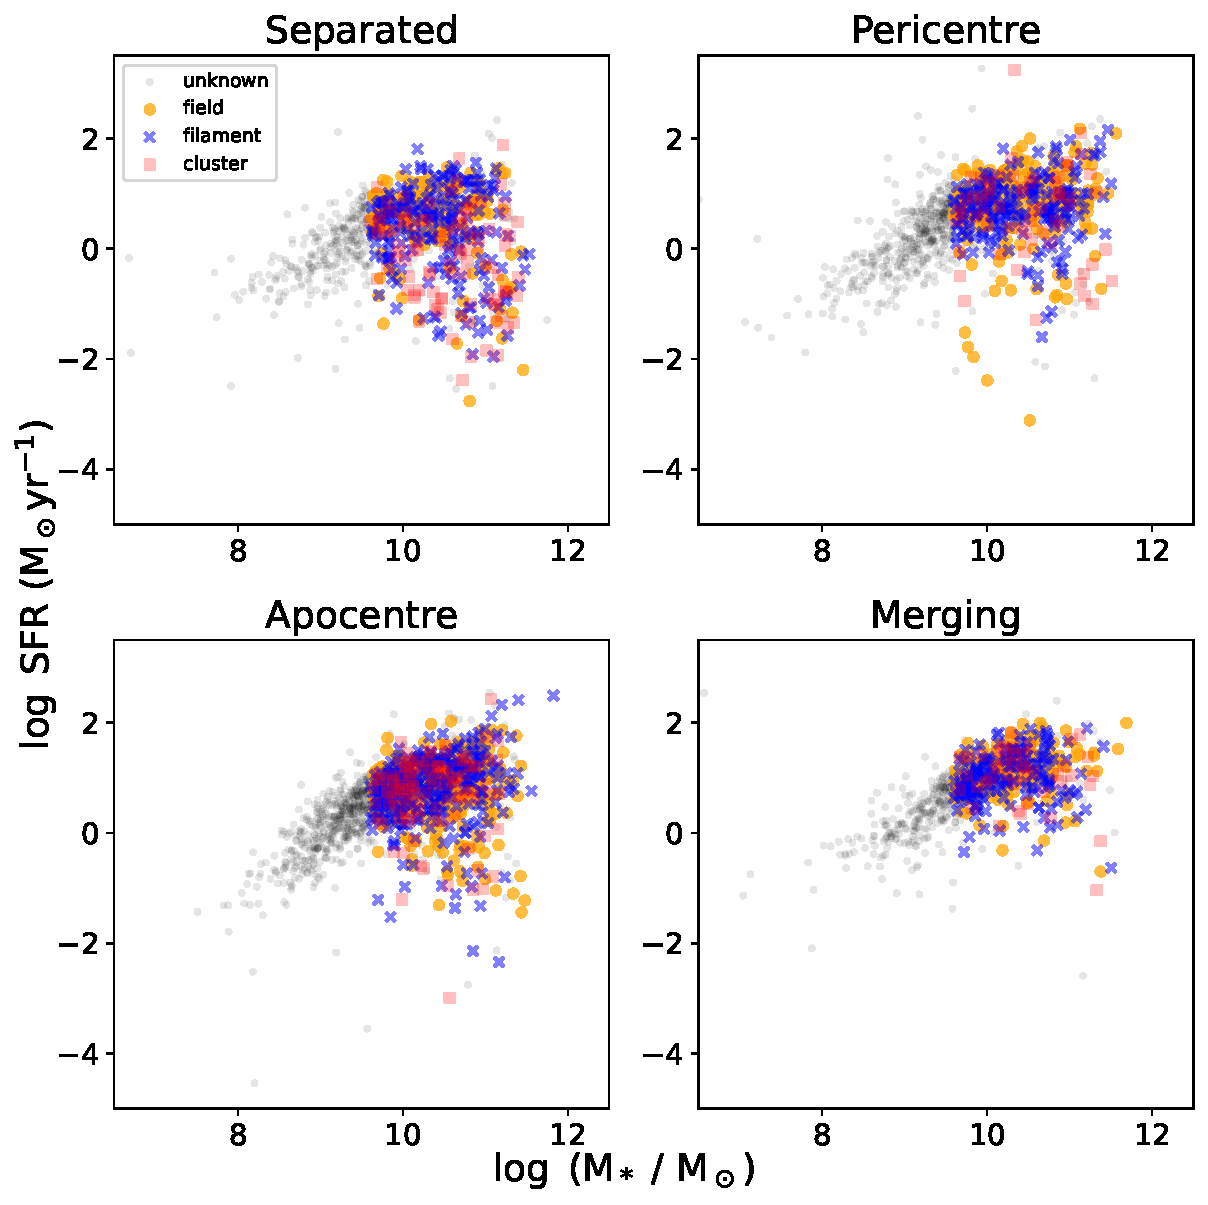
\includegraphics[width=\textwidth]{Chapter3/figures/sfr-mass-density.pdf}
\caption[The distribution of environment classifications through our sample.]{The distribution of environment classifications through our sample. This is only for sources with a $\log$M$_*$ / M$_\odot \geq$ 9.6. However, from this subsample, we see that there is no trend with environment and that the distribution is random throughout each stage.}
\label{fig:dens-sfr-mass}
\end{figure}

Another source that could be of major contamination is in our merging stage sample. We have identified the merging stage as those systems with a disturbed disk and containing more than one core. Another such system that could be recognised by this description is that of a clumpy galaxy. Clumpy galaxies are systems with internal regions undergoing intense star formation. These regions appear like multiple other `cores' throughout the galactic disk which are actually clumps of young stellar populations. To avoid such contamination, we apply multiple criteria to mitigate the potential impact they might have. First, our redshift range spans a sufficient range that the found fraction of clumpy galaxies declines rapidly compared to the merger rate \citep{2022ApJ...931...16A}. This is particularly true at $0.15 \leq z \leq 1$. Previous works have found the peak of the fraction of clumpy galaxies at $z\approx2$ \citep{2014ApJ...786...15M, 2018ApJ...853..108G}, well beyond our redshift range. There are also two morphological distinctions that we use to our advantage to discern between merging and clumpy galaxies. Clumpy galaxies often exhibit more than one clump at different radii across the galactic disk \citep[with][finding a mean of 3.16 clumps per galaxy]{2022ApJ...931...16A}, making them easy to differentiate from a second core which would be close to the centre of a perturbed disk. We therefore remove potential merging galaxies which appear to have more than one `core' at different places of a non-perturbed disk ($\sim25$). With the low fraction of clumpy galaxies in our redshift range and an increased number of cores compared to mergers we are confident we have separated out potential contamination by clumpy galaxies.

\subsection{Aside: Mass Ratios in Sample}
Here, we briefly discuss the mass ratios we find of our identified pairs of interacting galaxies. Figure \ref{fig:mass-ratio} shows the distribution of interaction types through our subsample. We find that our sample is dominated by micro and minor interactions.

\begin{figure*}
\centering
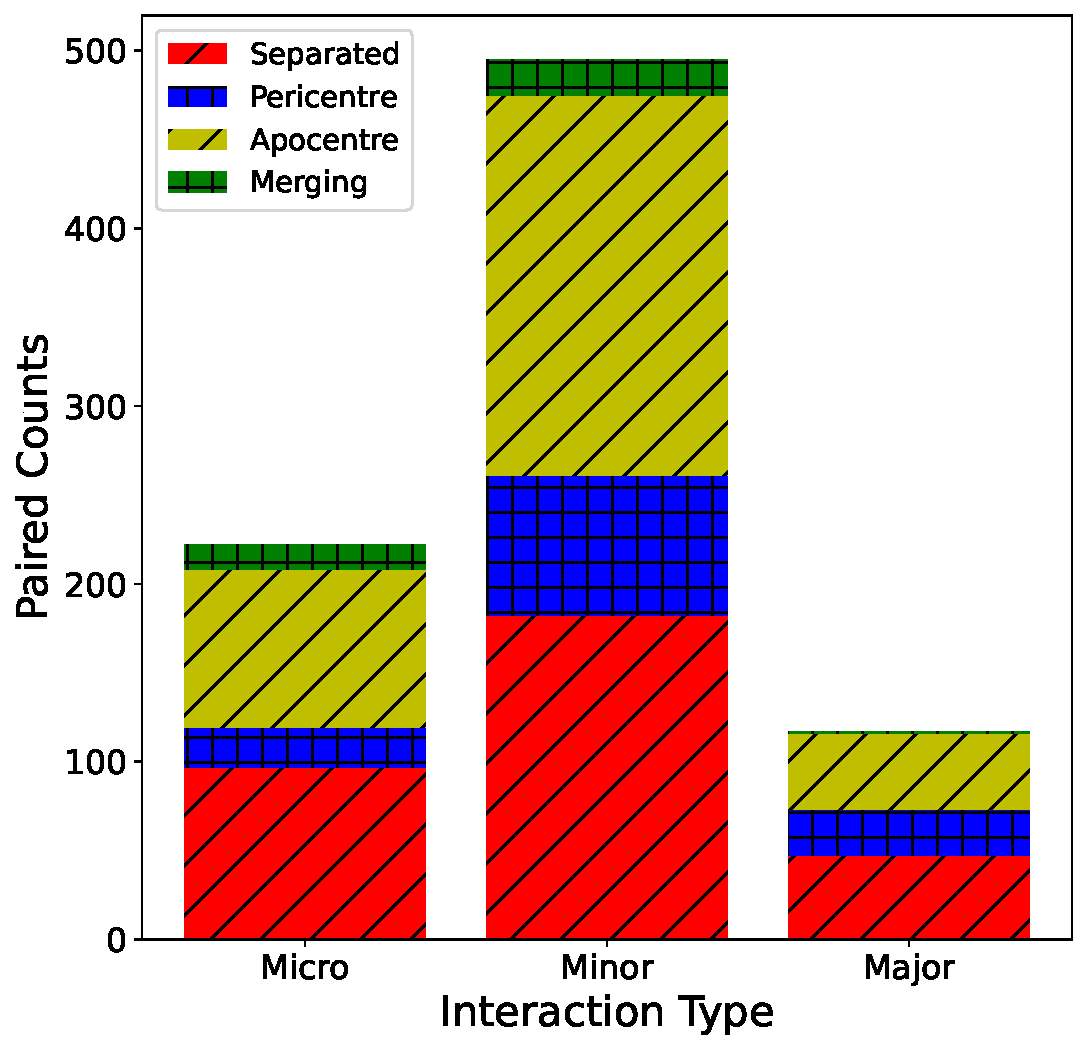
\includegraphics[width=\textwidth]{Chapter3/figures/mass-ratio-diagnostic.jpeg}
\caption[The distribution of mass ratios in our paired sample and across each stage of interaction.]{The distribution of mass ratios in our paired sample and across each stage of interaction. These are separated into our previously defined interaction stages and the interaction type (based on mass ratio). We find that, overwhelmingly, our sample is dominated by micro and minor interactions. These are where the two systems have very different stellar masses.}
\label{fig:mass-ratio}
\end{figure*}

The mass ratio is known to have a direct impact on the potential enhancements we see in SFR and in AGN fraction. While we do not focus on the mass ratio throughout this work, due to the limited pair galaxy size, knowing that we are dominated by micro and minor interactions will inform us of the relations we expect to uncover from our analysis. This assumes, of course, the subsample of galaxy pairs is representative. With this note on the distribution of interaction types based on mass ratio in mind, we now look at the relation between the stellar mass of our systems and the SFRs through interaction stage.

\section{Star Formation and AGN Evolution with Interaction Stage}\label{results:SF_stage}
\subsection{Controlling for Interaction Stage}\label{results:int_stage}
\noindent With our mass-limited sample selected, we investigate the change in multiple parameters with stage of the interaction. First, we show the results of breaking down our sample into stages with relation to the SFR and stellar mass of our sample. We use the estimates of these parameters that exist in the COSMOS2020 catalogue itself. Then, we use our subsample of galaxy pairs to recover the relationship between projected separation and star formation enhancement (SFE). We then further break this measure down into its component stages.

Figure \ref{fig:sfr-mass} shows the breakdown of stellar mass and SFR with stage. On a population scale, there is clear evolution in the star formation rate from the separated stage through to the merging stage. In the separated stage, where the galaxies are distinct from one another with no clear morphological disturbance, we clearly see two populations of galaxies. These are the blue, star-forming galaxies and red sequence of galaxies. The blue contours in Figure \ref{fig:sfr-mass} show increasing number density in the population into the blue cloud. In the pericentre stage, when the galaxies are actively interacting and overlapping, this red sequence remains but is highly diminished while there is no change in the blue cloud. The apocentre stage shows a similar effect, where the red sequence reduces again before finally in merging the red sequence completely disappears. Through these, the blue cloud remains highly populated and hosts the majority of galaxies in the stage.

\begin{figure}
\centering
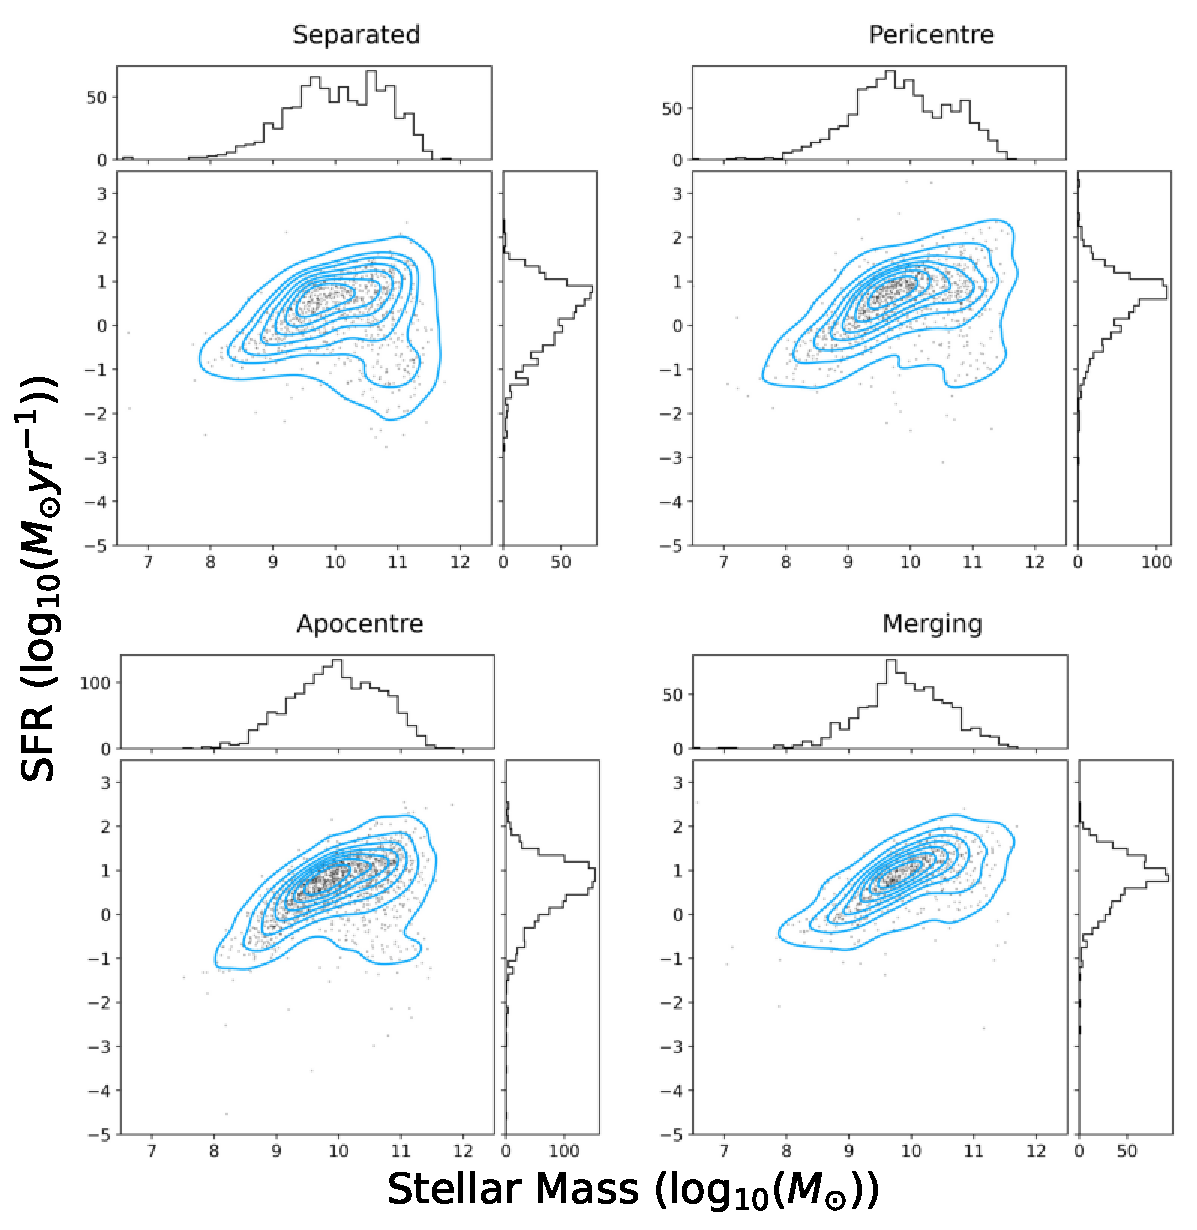
\includegraphics[width = \textwidth]{Chapter3/figures/sfr-mass-stages.pdf}
\caption[The \texttt{LePhare} stellar mass against the \texttt{EAzY} SFR across the different stages of the interaction.]{The \texttt{LePhare} stellar mass against the \texttt{EAzY} SFR across the different stages of the interaction. The blue contours are 8 levels of density of the underlying populations in each frame. \textit{Top left}: The stellar mass and star formation rate of the separated stage of our sample. Here, the interacting galaxies are simply close pairs with little to no morphological disturbance. There are clearly two populations here: a main, star forming sequence forming the main population and a smaller red sequence. \textit{Top right}: pericentre stage of the interaction, where the two interactors are close to pericentre. The star forming sequence remains, but the red sequence is reduced significantly. \textit{Bottom left}: apocentre stage of the interaction, where the interactors are close to apocentre or escaped. Here, we see the almost complete disappearance of the red sequence. \textit{Bottom Right}: merging stage of the interaction, where the two systems are close to or have coalescence. The red sequence of galaxies has completely disappeared.}
\label{fig:sfr-mass}
\end{figure}

However, this result could also be due to many other factors rather due to interaction stage. For instance, if the mass distribution of our sources evolves as well, we could simply be selecting higher mass systems as we increase stage. This would have the result of systems in the merging stage having, on average, higher SFRs than those in the separated stage and appearing like we had evolution in the star forming population with stage. Another effect that could cause this relation to appear would be our selection was highly dependent on galactic environment. However, we have already explored this possibility in Chapter \ref{data:environ} and found no bias in environment between the stages. Therefore, this is likely not the cause of this decrease in the red sequence population.

We can quantify the similarity of the mass distributions, and then the SFR distributions, using well known statistical tests. We opt to conduct tests: KS and AD-tests. First, we create weighted distributions of stellar mass. The weighting scheme we use balances the distributions such that each bin could be assumed to have the same number of sources within it. Therefore, any bins with fewer than a certain number of sources will be weighted up while those bins with more will be weighted down. These weights applied to the mass distribution are then applied to the SFR distribution as to control for stellar mass in this distribution.

\begin{figure}
\centering
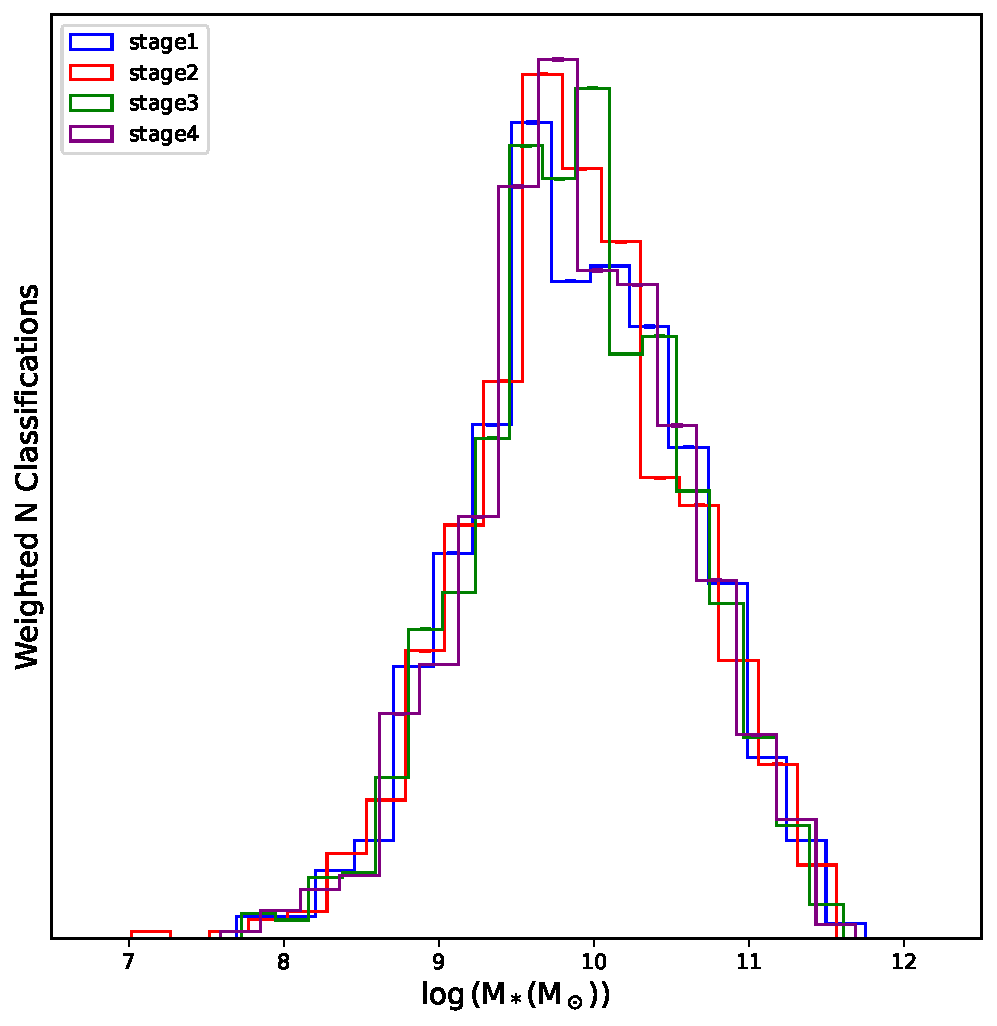
\includegraphics[width = \textwidth]{Chapter3/figures/stellar-mass-dist.pdf}
\caption[The stellar mass distribution across the four stages.]{The stellar mass distribution across the four stages. Each bin is weighted based on the counts in the smallest sub-sample in stage: the merging stage of the interaction.}
\label{fig:weighted-mass}
\end{figure}

\begin{figure}
\centering
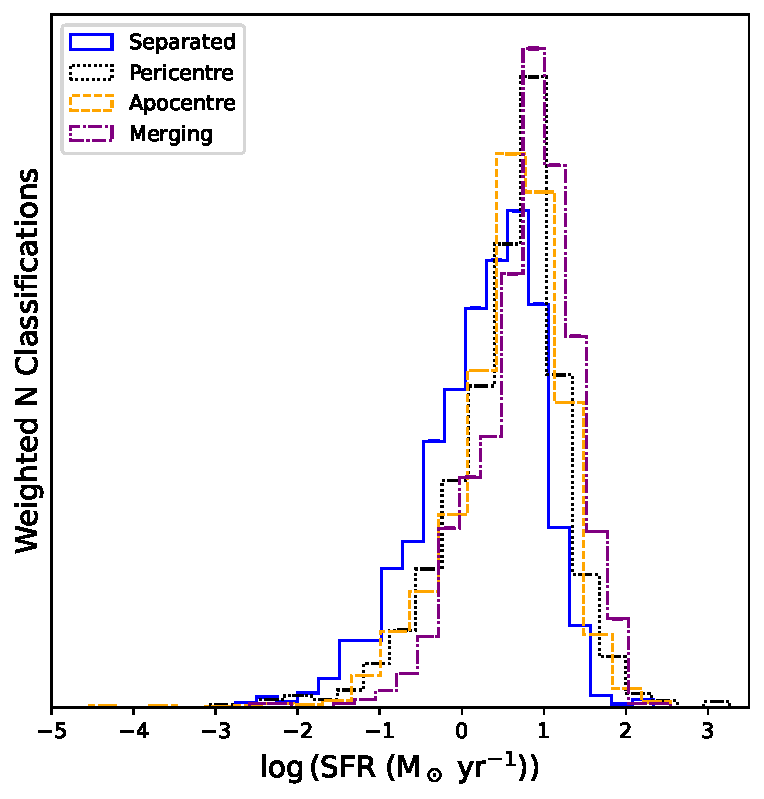
\includegraphics[width=\textwidth]{Chapter3/figures/sfr_dist.pdf}
\caption[SFR distribution weighted by mass across each stage.]{SFR distribution weighted by mass across each stage. This weighting is based on our sample of merging stage.}
\label{fig:weighted-sfr}
\end{figure}

Figure \ref{fig:weighted-mass} shows the weighted mass distributions through the four different stages. These appear similar, however, to statistically measure the similarity we apply our KS- and AD-tests to them. We chain the KS and AD test through each distribution and calculate the value of the test values and a $p$-value. This $p$-value represents the probability that each distribution is drawn from the same parent distribution. For each mass distribution, we find that $p$-value of both tests is $\approx1$. Thus, proving that the distribution in stellar mass though each stage is likely drawn from the same parent sample. 

Figure \ref{fig:weighted-sfr} shows the SFR distributions while being weighted by stellar mass. When comparing the separated and pericentre, separated and apocentre, separated and merging, pericentre and merging and apocentre and merging stages, the $p$-values are $\ll$0.05. This allows us to reject the null hypothesis for these distributions and assume they are from different parent samples. However, for comparing pericentre and apocentre stages, the $p$-value$=0.74$. Thus, while these distributions are likely to be not identical, they are very similar in the parent sample they have been drawn from. For the same mass distribution through each stage of interaction, the star formation distribution changes from separated to pericentre stage and from apocentre to merging stage, while remaining similar from the pericentre to apocentre stage. The errors on these distributions are calculated using the methodology of \citet{2011PASA...28..128C}. In this approach, we assume that the error about our measurements is simply a measure of the limited samples we have of the underlying beta distribution of the full population. Thus, we can measure the confidence intervals around our measurement by using the beta distribution. We calculate the 68.3\% confidence interval about our found value, and use the distance between these values as our upper and lower errors.

Putting this result into the context of the dynamical timescale of an interaction, it shows there are distinct points at which the SFR changes in these systems. The first is when the interacting system moves from being a close pair to actually morphologically disturbing each other in a close flyby. This difference, most likely enhancement, then persists through to the apocentre stage - where the galaxies remain highly disturbed but are no longer overlapping with their secondary. The SFR distribution remains approximately the same between these two, meaning the forces that drive and affect star formation remain equivalent between these two stages. Finally, the SFR changes again when we approach the merging or post-merger stage of the interaction. We can also say that this change is likely an enhancement in the SFR of the galaxies through the interaction due this change being driven by the disappearance of the red sequence through each stage.

We further examine this result by controlling for redshift and making specific classifications of galaxy star formation class. While the red sequence is significantly reduced across across each stage, it is difficult to ascertain the change in the galaxies within the blue cloud. We expect that, due to an interaction, the population of starbursting and quiescent galaxies will change. Therefore, we define a star forming main sequence (SFMS) across redshift. This allows us to classify each source based on its SFR independently of redshift. To define the star forming main sequence, we follow the example of \citet{2019MNRAS.484.4360A}. There, they define the star forming main sequence as a function of galactic stellar mass and redshift as

\begin{equation}
\log \text{SFR}_{\text{MS}}(z)[M_\odot yr^{-1}] = -7.6 + 0.76\log\frac{M_*}{M_\odot} + 2.95\log(1+z).
\end{equation}

\noindent This finds the expected main sequence SFR of a galaxy at a given stellar mass, $M_*$, and redshift, z.

The ratio of the measured galaxy SFR and the expected main sequence SFR is then taken. We then use this fraction to classify each galaxy into distinct bins. These bins are:

\begin{enumerate}[(i)]
\item Starburst galaxies. Here, the galaxy SFR is highly elevated compared to the SFMS. We follow \citet{2019MNRAS.484.4360A} and define a cutoff of $\log$ SFR/SFR$_{\text{MS}} >$ 0.4.
\item Main sequence galaxy. The galaxy is within 0.4 dex of the SFMS and approximately has the expected SFR. Defined as $-0.4 < \log$ SFR/SFR$_{\text{MS}} < 0.4$.
\item Sub-main sequence galaxy. A galaxy whose SFR is below the majority of the SFMS, but likely not quiescent. Defined as $-1.3 < \log$ SFR/SFR $_{\text{MS}} < $ -0.4.
\item Quiescent (High) galaxy. A galaxy with an SFR in the top $\approx$50\% of the quiscent galaxy population. Defined as $-2.3 < \log$ SFR/SFR $_{\text{MS}} <$ -1.3.
\item Quiescent (Low) galaxy. A galaxy with low SFR and very likely completely quenched. Defined as $\log$ SFR/SFR$_{\text{MS}} <$ -2.3.
\end{enumerate}

\noindent We split our sample into its different stages and apply these criteria. Figure \ref{fig:sfr-clsf} shows the ratio between the expected SFMS SFR and the measured SFR in COSMOS2020. This clearly shows a large increase in galaxies classified as starburst from the separated to merging stages and a large reduction in the number of quenched systems. Figure \ref{fig:sfr-clsf-bar} shows the change in fraction of the different galaxy classifications through stage, reflecting the results found in Figure \ref{fig:sfr-mass}. Initially, in the separated stage, we find that the majority of our galaxies lie on the SFMS or just below it. There also exists a small population of galaxies which are classified as starburst with a population of quiescent galaxies that is roughly double the starburst fraction. As we move through the interaction stage, we see that the quiescent galaxy fraction gradually decreases to the point of almost non-existence in the merging stage galaxies. The inverse is true in our starburst fraction. We find this almost quadruples over the course of the different stages of interaction. The fraction of galaxies on the SFMS remains dominant throughout, however, we do find the fraction of sub-MS galaxies significantly reduced. We find that, in general, the SFR of these galaxies is increasing with interaction stage (though, not in the pericentre to apocentre stage). It appears to have sub-MS and quiescent galaxies move up and join the SFMS (as it remains dominant). But, many galaxies from the SFMS are moved upwards and into a starbursting phase.

\begin{figure}
\centering
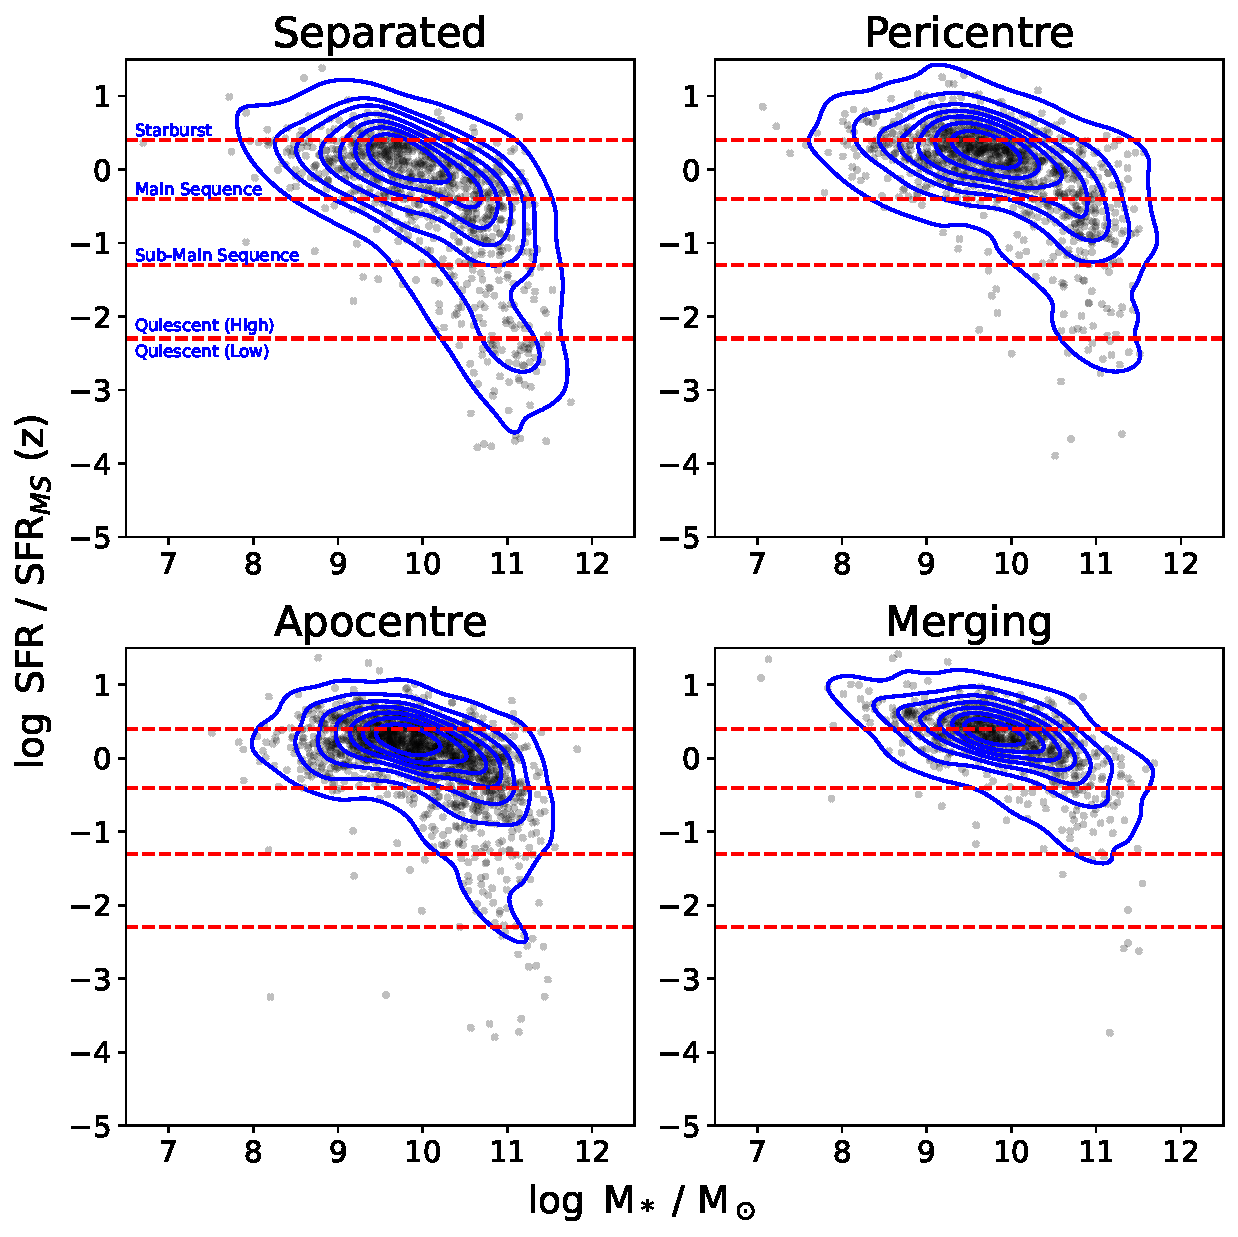
\includegraphics[width=\textwidth]{Chapter3/figures/sfr-clsf-dist.pdf}
\caption[Stellar mass against the ratio of measured SFR to the expected SFR if the galaxy was on the SFMS.]{Stellar mass against the ratio of measured SFR to the expected SFR if the galaxy was on the SFMS. Black points are the individual sources, while the blue contours are as in Figure \ref{fig:sfr-mass}. The red dotted lines show the cutoffs for different galaxy classifications based on their SFR, with each cut off being defined by the text in blue. The histograms beside each plot show the change in counts. We find that through interaction stage, the quiescent galaxy population significantly reduces while the starburst population rapidly increases. As these cutoffs are also dependent on redshift, we find that this evolution in SFR with interaction stage is independent of redshift.}
\label{fig:sfr-clsf}
\end{figure}

\begin{figure}
\centering
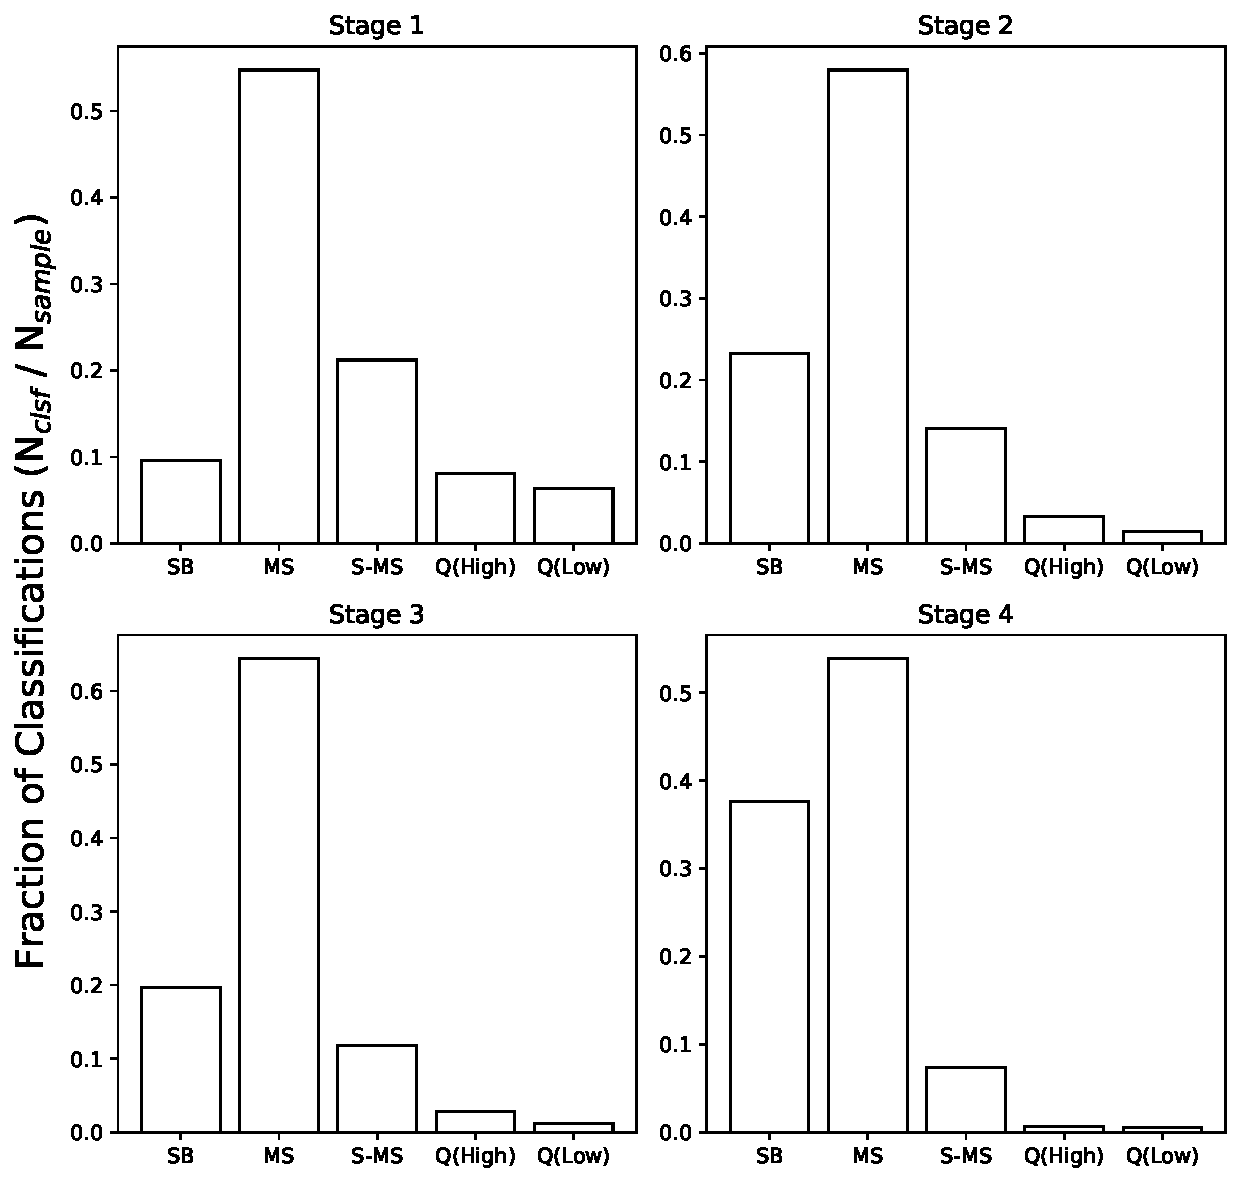
\includegraphics[width=\textwidth]{Chapter3/figures/sfr-clsf-bar.pdf}
\caption[The change in fraction of different galaxy classifications from the fraction of SFR to the expected SFR on the SFMS.]{The change in fraction of different galaxy classifications from the fraction of SFR to the expected SFR on the SFMS. While galaxies on the SFMS remain dominant through each sample across interaction stage, there is significant change in the starburst and quiescent populations. The starburst galaxy population moves from being roughly half the size of the quiescent population in the separated stage to completely dominating it in the merging stage. This is occurring while the quiescent population is significantly reduced to almost non-existence in the merging stage.}
\label{fig:sfr-clsf-bar}
\end{figure}

It is important to note the parameter space that we are searching in these examples. We are probing interactions between galaxies of high mass, where the resultant tidal features that form would be classifiable in an image. The majority of our sample is minor interactions where one of the two systems is very highly perturbed by the interaction. In this parameter space, we would expect large increases in the SFRs. However, we do not see a significant increase in the starbursting population until we the two galaxies begin to actually coalesce. Thus, the effect of the interaction itself may be to only enhance the SFR, while at coalescence we find the dramatic starburst. This can be argued from our results of clear, statistically robust change and evolution of a galaxy's SFR with interaction stage. The SFR changes dramatically from the separated to pericentre stage and apocentre to merging stage - after the initial passage of closest approach and at the point of coalescence of the interaction.

\subsection{Projected Separation and Star Formation Enhancement}
\noindent We directly investigate the relation between the SFE and the projected separation using our confirmed sub-sample of galaxy pairs. This sample is significantly smaller than our non-pair sample: containing 338 pairs or 676 galaxies (we have also added some pairs from the additional interacting galaxy sample). Upon sub-dividing this into different stages we find 228 separated galaxies, 102 pericentre galaxies and 342 apocentre galaxies. Only 4 merging galaxies were in our confirmed galaxy pair sub-sample, and therefore we do not attempt to make inferences about this population. 

To measure the SFE of our galaxy pairs, we directly compare to the mass- and redshift-matched control sample that was also created with this sub-sample and defined in Chapter \ref{sec:sec-ident}. We separate our galaxy pairs into different bins based on the projected separation between them. We find that the bulk of our sample has a projected separation between the two galaxies of $\leq$50kpc. Therefore, we sample from this region of the parameter space with high precision and smaller bin widths before we increase the bin widths at larger projected separations. We define a cutoff that each bin must contain at least 10 counts to be included in this plot and, therefore, by changing the bin widths with projected separation we are able to maintain some level of statistical robustness. We define our bins as [0.5, 10, 20, 50, 100, 125] kpc.

We create two projected separation distributions: one of interacting galaxies and the other of our control galaxies. We then take the average of each bin. By taking the average of each bin, we find the total excess of the SFR caused by interaction alone and then compare it to what we would expect from non-interacting galaxies in the same bin. Note that the control galaxy relation to the projected separation is meaningless as they are not paired. The control galaxies are simply mass and redshift matched to each interacting galaxy and used as a reference for what SFR we would expect of it had it not been interacting. Finally, we divide the averaged interacting SFR distribution by the averaged control SFR distribution. This provides us with a measure of the excess star formation due to interaction, and the SFE when compared to the isolated population.

\begin{figure*}
\centering
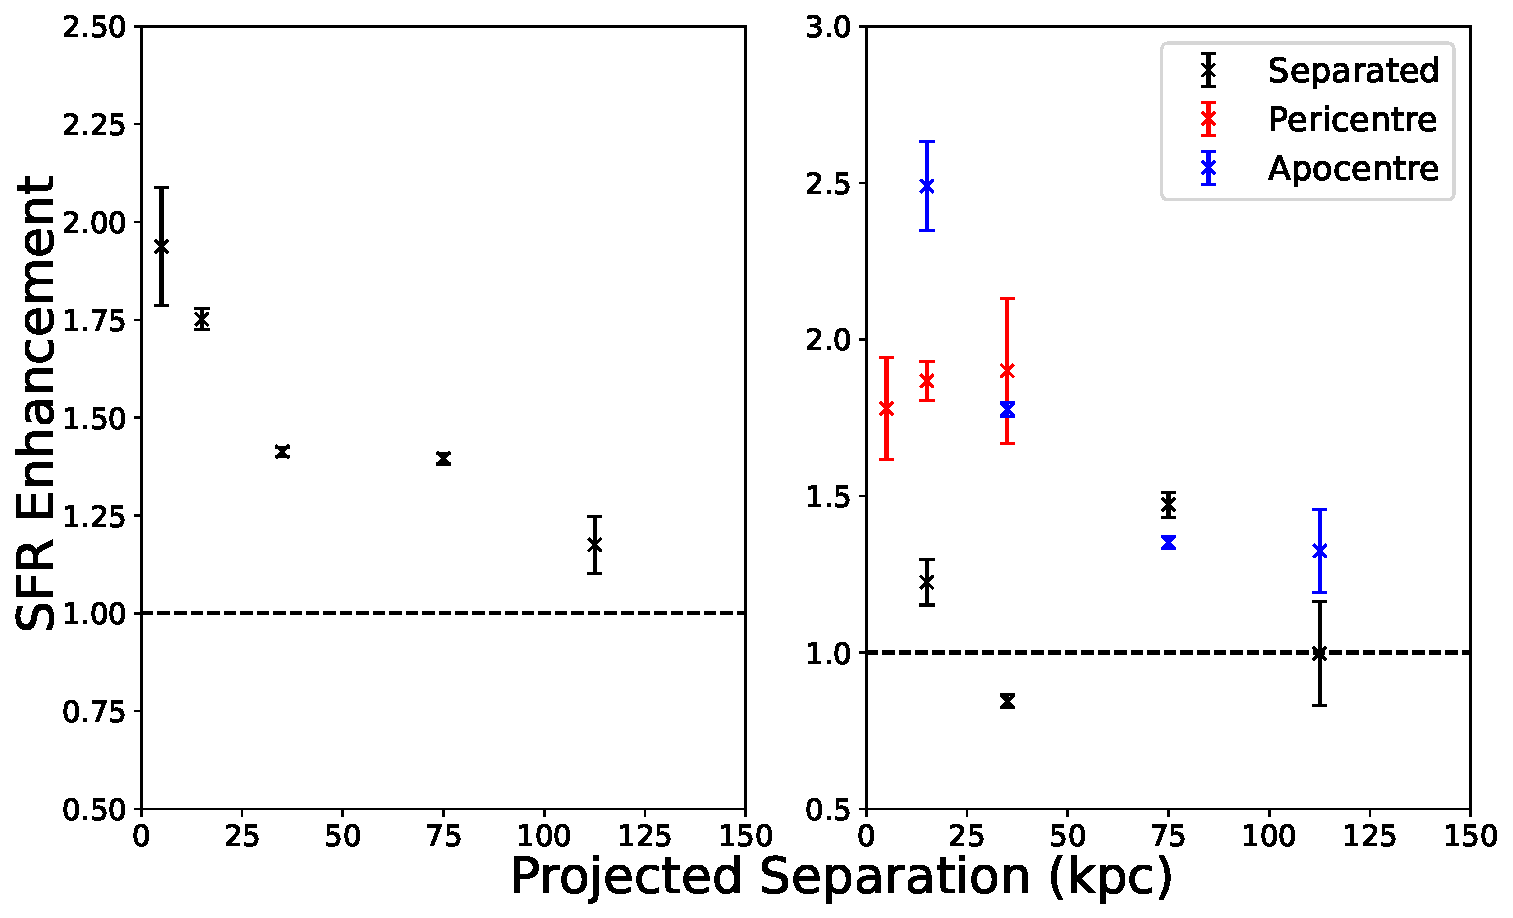
\includegraphics[width=\textwidth]{Chapter3/figures/sfr-enhancement-projected-sep.pdf}
\caption[The projected separation against the SFE in average star formation at different bins of projected separation.]{The projected separation against the SFE in average star formation at different bins of projected separation. Each bin must contain at least 10 counts to be considered. As the bulk of our galaxy pair sample is at low projected separation, we heavily sample from this region of the parameter space. The bins are: [0.5, 10, 20, 50, 100, 125] kpc. As we move to higher projected separation, the bins increase in width to maintain statistical significance in our sample. \textit{Left}: The star formation enhancement found in the entire galaxy pair sample. As expected, we see a gradually decreasing enhancement. \textit{Right}: As left but broken up into different stages of the interaction. Black markers are the separated stage, red the pericentre stage and blue the apocentre stage. We limited our investigation to the separated, pericentre and apocentre stages as only three galaxy pairs were identified in the merging stage. We find a generally decreasing star formation enhancement with projected separation but very different individual behaviour dependent on the stage classification.}
\label{fig:sfr-enhancement-sep}
\end{figure*}

Figure \ref{fig:sfr-enhancement-sep} shows star formation enhancement between our interacting and control binned SFRs and the projected separations between each galaxy pair. On the left of the plot, we have the distribution for the full galaxy pair sample, without taking account of stage. The errors on our measurements are following the methodology of \citet{2011PASA...28..128C} and briefly described in Chapter \ref{results:int_stage}. The dashed black line represents no enhancement in SFR, as the average SFR in the interacting galaxy sample would be equal to the average SFR in the control sample. We find at very small projected separation a SFR enhancement of 1.74 which gradually decreases with projected separation down to approximately 1 at 117.5kpc. 

On the right, we break the galaxy pair sample into different stages and plot out the resultant enhancement in star formation. This shows very different behaviour in enhancement dependent on the stage of the interaction. In the separated stage, we find that the star formation is very weakly enhanced, and with no overall structure. The enhancement moves around 1 through the distribution, with some enhancement being a result of low number counts in the bin. This is not unexpected. The separated stage represents when the two galaxies are close pairs, but with no morphological disturbance. Therefore, we would not expect significant, if any, enhancement in the SFR based on the projected separation. This is the stage with the lowest enhancement across projected separation.

In the pericentre stage, we see consistent enhancement with projected separation. It is also much larger than the separated stage, with it being approximately 1.6. In fact, the measured enhancement increases across the 50kpc of projected separation. However, accounting for the errors on these measurements and the declining counts in each bin, it is likely that the enhancement remains constant as the projected separation increases. We see a very large enhancement in the overlapping apocentre stage galaxies which overlap with the pericentre stage measurements. The enhancement in apocentre stage galaxies then rapidly declines as we move to higher projected separations. After 150kpc, our galaxy pair sample does not have the counts to make robust estimates of the SFE. However, it is important to note that this result has been found with a sample of 676 interacting galaxies in their pairs. No merging stage galaxies have been represented and in numerous projected separation bins the counts are small enough to have conclusion altering error bars. Therefore, it is imperative that future works, with larger sample sizes not only look at the projected separation of the systems but the morphology as well.

\section{Nuclear Activity with Interaction Stage}\label{results:AGN_stage}
\noindent We now use our AGN sample matched with the AGN catalogues described in Chapter \ref{sec:agn-clsf}. As stated previously, we find matches of 1,361 AGN and star forming galaxies (SFGs). The breakdown of number of classifications per stage is shown in Table \ref{tab:agn-sfg-breakdown}. Figure \ref{fig:agn-stage} shows distribution of stellar mass to SFR with stage, with the confirmed AGN and SFGs marked. We find no major changes in AGN with stellar mass or SFR with stage in our sample. Galaxies containing AGN appear throughout the starburst, the SFMS and red sequence across each stage. There is no obvious bias in stellar mass or SFR for hosting an AGN. We do, however, see a concentration of AGN in the separated stage on the red sequence at higher masses. This changes as we increase interaction stage, with the bulk of the AGN beginning to appear at lower masses in the apocentre and merging stages. Finally, in the merging stage we see AGN and SFGs distributed almost evenly across the star forming main sequence with little bias in distribution with mass.

Applying KS or AD tests to these, however, reveals $p$-values close to 1 and therefore these distributions are consistent with being drawn from the same parent sample. However, due to the low counts of AGN and SFGs in our sample, using KS and AD tests to verify this is not optimal. Therefore, we instead investigate the global AGN fractions in our sample across different stages. We apply a weighting, as in our SFR and stellar mass distribution examples, to account for the various counts across the different stages. We then take a second weighting of the measured AGN fraction from the total size of the different samples we have. Thus, we have assumed that we have equivalent counts in each mass bin of our sample as well as approximated having the same sample size in each stage bin.

\begin{figure}
\centering
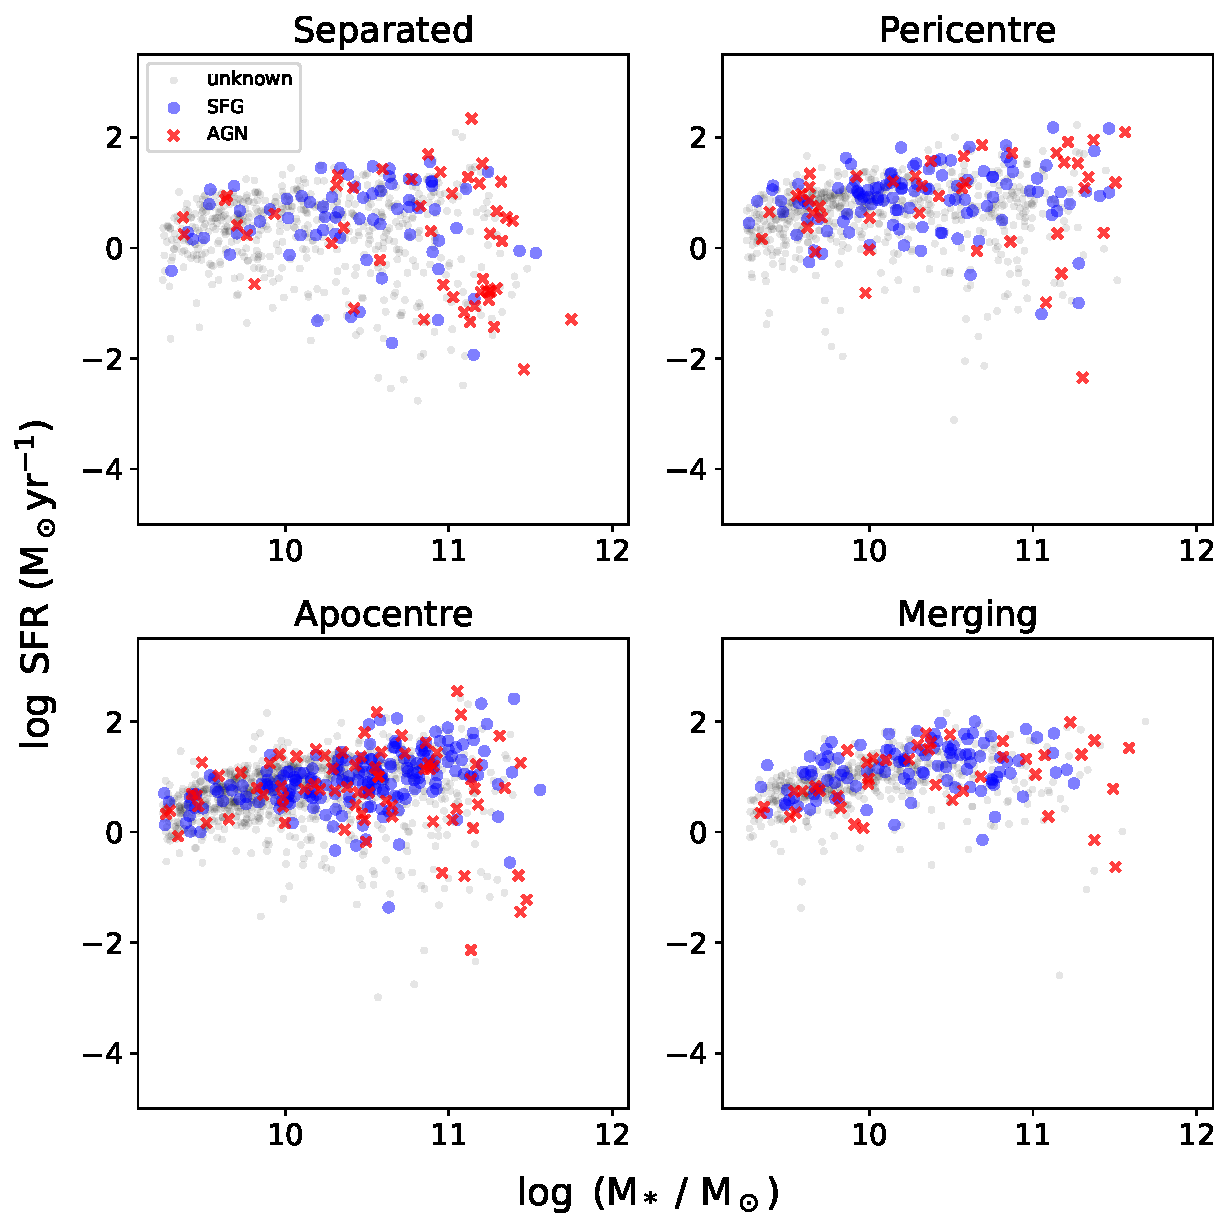
\includegraphics[width=\textwidth]{Chapter3/figures/agn-stage-dist.pdf}
\caption[The distribution of AGN through stage with SFR and stellar mass.]{The distribution of AGN through stage with SFR and stellar mass. We find that the AGN populate every part of the SFR-M$_{*}$ parameter space probed in the pair sample.}
\label{fig:agn-stage}
\end{figure}

\begin{table}
\centering
\begin{tabular}{|c|c|c|c|c|}
\hline
& Separated & Pericentre & Apocentre & Merging \\
\hline
SFG & 135 & 212 & 337 & 199 \\
AGN & 103 & 117 & 163 & 95 \\
\hline
\end{tabular}
\caption{Breakdown in number of classified AGN and SFGs per stage. With our counts so low in this sample, it is difficult to make concrete conclusions about the evolution of AGN during interaction.}
\label{tab:agn-sfg-breakdown}
\end{table}

\begin{figure}
\centering
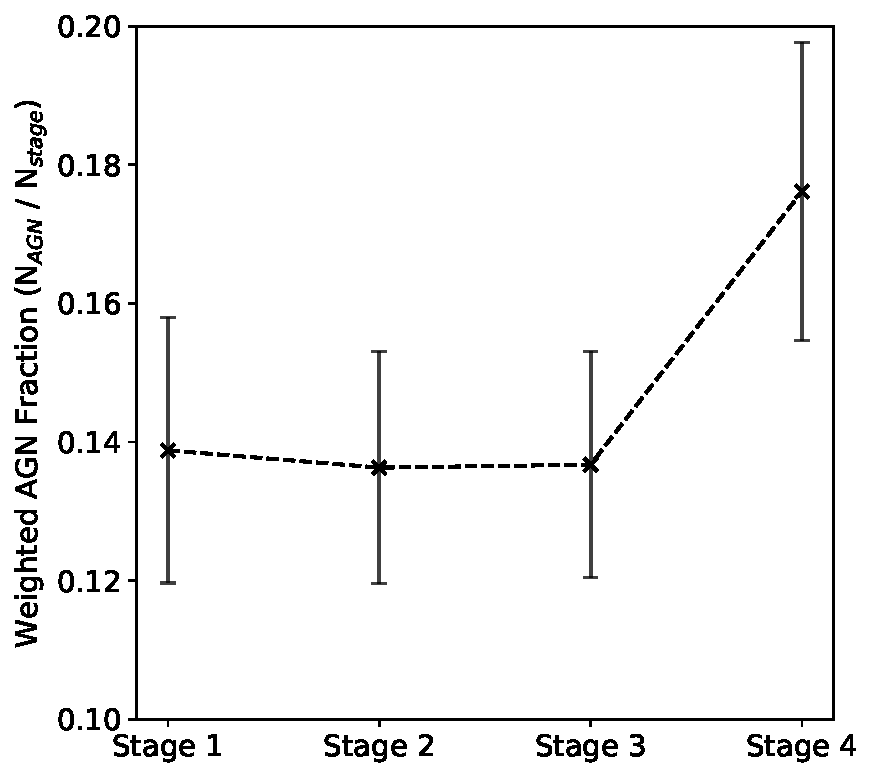
\includegraphics[width=\textwidth]{Chapter3/figures/agn-frac-time.pdf}
\caption[The change in AGN fraction with stage.]{The change in AGN fraction with stage. The dotted line is the expected AGN fraction in the field (from \citet{2008AJ....135.1877E}). We define the AGN fraction as the ratio of number of confirmed AGN divided by the number confirmed AGN and SFGs in the sample. This is then weighted by the relevant sizes of each subsample and the number of unclassified sources in each. Errors on each fraction are found as the confidence intervals defined via the beta distribution. We find a sudden drop in AGN fraction from the separated to pericentre stage, followed by a rapid increase from the apocentre to merging stage.}
\label{fig:agn-frac-time}
\end{figure}

Figure \ref{fig:agn-frac-time} shows the changing AGN fraction with interaction stage. The dotted line shows the expected fraction of AGN in the field from \citet{2008AJ....135.1877E}. We find that the AGN fraction generally remains at the fraction of the field through the separated to apocentre stages. There is a small decrease from the separated to pericentre stage, followed by the fraction mostly remaining unchanged until the apocentre stage. Then, in the merging stage we measure a large increase in the AGN fraction from $\approx0.12$ to $\approx0.15$, far above the expected field fraction. However, before we discuss this result further, we must point out that the large error bars on our measurements and the low number counts of confirmed AGN and SFG make this difficult to interpret.

% Section here on actually looking at the projected separation of the two systems.
It is also difficult to use interaction stage as a proxy for the projected separation in this context. As shown previously, the pericentre and apocentre stages have some overlap in the range of projected separations we have classified them into. Therefore, we also investigate any overlap between our confirmed pairs and the AGN fractions we see here. We find 104 AGN and 180 SFGs overlap with our confirmed pairs. Figure \ref{fig:sfg-agn-proj} shows the change in density of AGN classifications and SFGs with increasing projected separation. As expected, we find that with increasing projected separation the number of confirmed AGN and SFGs decreases. In the AGN distribution, we find two contributing components in it. The first is a peak in the projected separation distribution is from 0kpc-25kpc. The only contribution here is from pericentre stage galaxies. The second peak, from a projected separation of 30kpc - 60kpc is dominated by apocentre stage galaxies, although some separated stage AGN are in this peak as well. Finally, the third peak from 85 - 125kpc is representative of a mixture of the separated and apocentre stage galaxies. None of our merging stage galaxies which had their secondaries identified overlapped with our AGN and SFG identified sample.

\begin{figure}
\centering
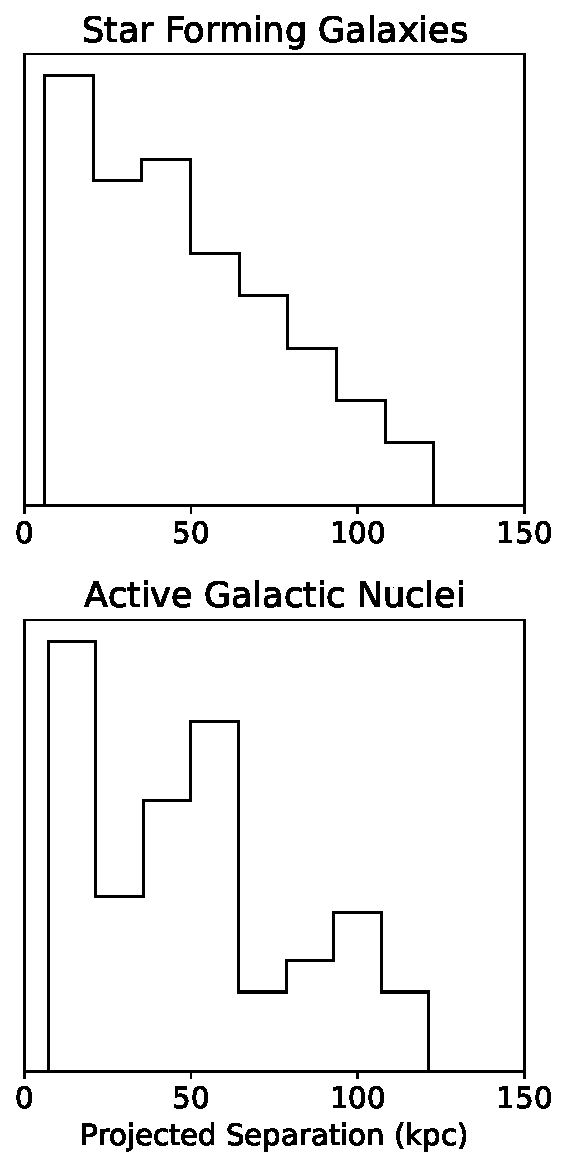
\includegraphics[width=0.58\textwidth]{Chapter3/figures/sfg-agn-dist.pdf}
\caption[The distribution of both AGN and SFGs which have been matched our confirmed galaxy pairs.]{The distribution of both AGN and SFGs which have matched our confirmed galaxy pairs. While we find, as expected, the number of AGN and SFGs decreases with projected separation we find an interesting double peak in the AGN sample. The first peak, between a projected separation of 0 and 25kpc is primarily from pericentre stage galaxies (in red) while the second peak of 40 to 65kpc is of apocentre stage galaxies (in yellow) in our sample. As shown in Figure \ref{fig:agn-frac-time}, we expect the fraction of AGN to be similar in these two stages despite being at different parts of the dynamical timescale in interaction. The third peak, from 75 to 125kpc is only from separated and apocentre stage galaxies.}
\label{fig:sfg-agn-proj}
\end{figure}

We find the AGN fraction only increases at the point of coalescence in interaction: the merging stage. This indicates that the mechanism driving AGN ignition in interaction is primarily at the point of the closest approach between the two systems. When we investigate the AGN number counts with respect to the projected separation of systems, we find that it gradually declines over the projected separation. However, we find two peaks; first clearly in the pericentre of the interaction where the galaxies are overlapping and secondly in the early parts of the apocentre stage. This could be evidence of a delayed AGN ignition depending on the underlying parameters of the interaction. Thus, we find that the AGN fraction is generally unchanged with stage, although the mechanisms responsible for an increase in the fraction primarily occur when the two systems are actually merging. We find evidence of a delay of ignition, as there is a peak in AGN counts at a small projected separations in the apocentre stage.

\section{Discussion}\label{discussion}
\subsection{Interaction Stage and Projected Separation}
\noindent Finding evolution with interaction stage is not a new idea in the field. Multiple works have found increases in SFE and SFR as a function of projected separation of pairs of galaxies \citep{2000ApJ...530..660B, 2008AJ....135.1877E, 2013MNRAS.433L..59P}. Projected separation is often seen as a proxy for the point in the dynamical time of the interaction that is being measured. It is likely that, when the galaxies in the pair are closer together, they are closer to coalescence in the dynamical time and can be thought of as a linear progression in the interaction from being close pairs to coalescence. However, what this fails to capture is the larger complexity of interaction. Without morphological consideration, we are unable to tell whether galaxies at small projected separations are actually at the closest point of flying by each other or about to coalesce.

We find that throughout the different stages of interaction the SFR within the systems is increasing. Observations of interacting galaxies at various stages have found increased gas inflows into the nuclear regions of the galaxies which lead to enhancement in the SFR at the galactic core over their outer reaches \citep{2015A&A...579A..45B}. This is often confirmed with deep observations of individual systems, which capture snapshots of different parts of the dynamical timescale of the interaction \citep{2022MNRAS.514.2769K}. Our study utilises numerous snapshots of the dynamical time of interaction in attempt to build a full picture of the change in SFR. We have found that this process increases the SFR of galaxies and that being driven to starburst begins from the pericentre of interaction. Multiple simulation works, which have the ability to model the entire dynamical history, show that this is to be expected \citep{2007A&A...468...61D, 2013MNRAS.430.1901H, 2015MNRAS.452.2984K, 2021MNRAS.503.3113M}. Often, these works show an initial dramatic increase in the SFR of interacting systems followed by an exponential decline through the dynamical time before increasing dramatically again at either a second passage or coalescence. \citet{2015MNRAS.448.1107M} is a direct example of this SF history through the interaction.

Our results differ here as we do not find an exponential decrease in the SFR as move from the pericentre systems to the apocentre systems. As stated previously, observational work does support a continued increase in SFE in galaxies to projected separations of out to 80kpc - well into our defined apocentre stage systems \citep[for further examples, see][]{2008MNRAS.385.1903L, 2012MNRAS.426..549S}. However, it is important to note that our apocentre stage defined classification is a `wide net' that captures many systems that may be very soon after the initial passage in the dynamical timescale (recall Figure \ref{fig:illustration}). The criteria defining pericentre and apocentre stages are simply that the galaxies must be no longer connected or overlapping morphologically with tidal features. They must only be distinct and separate galaxies. Therefore, our found large enhancement in the apocentre stage may be from interacting systems which are only just out of the pericentre passage and not enough time has passed for the rapid decline in SFR to begin. 

Nonetheless, we still find a disappearance of the red sequence in the apocentre systems which may come as unexpected to when compared to simulations. It is important to note, however, that this is not the same as saying that a large proportion of the apocentre systems are classified as starbursting galaxies. While previously mentioned simulations approximate an initial large starburst before rapid decline, we find the interacting galaxy population is pushed from being quiescent / sub forming main sequence to being on the star forming main sequence. Therefore, it may be more likely that the impact of interaction on star formation is not to suddenly cause rapid star formation in the aforementioned starburst before declining, but rather to gradually increase a galaxy's SFR up and into the blue cloud of galaxies. This could be supported by the lack of rapidly quenched post-interaction galaxies found in both observations \citep{2017ApJ...845..145W} and simulations \citep{2020MNRAS.493.3716H, 2021MNRAS.504.1888Q}. Thus, the impact of interaction on star formation may not be a catastrophic increase in star formation that leads to quenching but, rather, a small increase in galaxies to use whatever gas they have into star formation. % Expand?

This idea can be brought further forward by considering the large increase in starbursting galaxies we find when going from pericentre / apocentre stage to the merging galaxies. The merging stage represents, in our sample, galaxies that are undergoing the final coalescence of the two systems involved. We find that the point of final coalescence leads to a large increase in the fraction of starbursting galaxies as well as the almost complete disappearance of the quiescent and sub-main sequence fraction of galaxies. Thus, from this result we can conclude that during coalescence galaxies undergo a huge starburst and enhancement in star formation which will quickly lead to their quenching. This is also supported by works such as \citet{2022MNRAS.517L..92E}, which find that galaxies post-coalescence are 30-60 times more likely than control galaxies to have rapidly shut down star formation.

Thus, we can conclude that, for merging galaxies if gas is present within them, star formation will increase and change our classification of the galaxy. We will observe a sudden increase in the star formation rates of these systems followed by a rapid quenching as the gas is used up entirely. This differs from galaxies that move into the apocentre stage and do not merge. These apocentre stage systems will then slowly lose their enhancement over a long period of time, and return to star forming at their expected rate, whereas only moving into a merging stage galaxy will lead to a starburst which may incur rapid quenching.

Such a conclusion would also, therefore, explain the often quite large divide in the literature between whether interaction actually leads to enhancement or not. The only part of the interaction which causes the enhancement, and is the forking point, is the pericentre stage. From this point, if the galaxies then move off to the apocentre stage and escape, we will see a gradual decline in the SFE with the apocentre stage galaxy only having a minor increase in its star formation classification. Whereas if the galaxies move into the merging stage of the interaction and coalesce we see the results of a major starburst and the complete using and of all the gas in the systems. Thus, leading to a large fraction of quenched post-merger galaxies, but only after the initial coalescence. 

\subsection{Interaction Stage and AGN}
\noindent The evolution of the AGN fraction in interacting galaxies is similar to that of the evolution of star formation. It has often been found with projected separation the AGN fraction increases. There are multiple observational works that show this \citep{2007MNRAS.375.1017A, 2013MNRAS.435.3627E, 2020ApJ...904..107S} as well as works on cosmological simulations which support these conclusions \citep{2023MNRAS.519.4966B}. In simulations, the increased likelihood of AGN activation comes from the sudden increase in gas density in the galactic core which naturally leads to increased black hole feeding, growth and nuclear activity. To satisfy these conditions, actual coalescence of the two systems are required. Observations of interacting galaxies are often interesting, as they contain examples of dual AGN and individual examples \citep[e.g.][]{2017MNRAS.470L..49E, 2021ApJ...923...36S} or investigate the increase in the AGN fraction in only the merger / post-merger stage \citep{2020A&A...637A..94G}.

We find peaks in the AGN fraction with projected separation, before the galaxy merging and coalescence takes place. This is supported with other works which specifically look at AGN fraction with projected separation \citep{2011MNRAS.418.2043E, 2023ApJ...942..107S}. However, we specifically find that the AGN fraction increases rapidly in the merging stage and holds quite constant between the separated to apocentre stages. This shows two distinct effects of interaction which can colour our interpretation of the link between AGN and interaction. It appears from our results that the AGN fraction is driven up during the points in the dynamical time when the inner parts of the galaxy are majorly disturbed, and not by the simple movement of gas and dust into the core during the two galaxies passing each other. There is evidence that the onset of nuclear ignition from interaction may be delayed \citep{2011MNRAS.418.2043E}, or even flicker \citep{2015MNRAS.451.2517S} after ignition. Both of these possibilities are reflected in the double peaked distributions of AGN fraction with projected separation and the different times in the dynamical time these represent.

Again, it is important to note the rather `wide net' that our stage classification takes. There is overlap between our pericentre and apocentre stage classifications at high pericentre projected separation and low apocentre projected separations. However, these stages naturally lead onto one another. Therefore, what see in the bi-modal distribution of AGN fraction with projected separation in Figure \ref{fig:sfg-agn-proj} are two peaks. The second of these peaks is at the cross over point of pericentre to apocentre; the point at which (if the two galaxies have just flown by each other) a delayed AGN ignition could take place. This is also reflected in Figure \ref{fig:agn-stage} where we see a slight increase in AGN fraction in the apocentre stage. This is likely from the ignition of nuclear activity taking place over a large period of time with a delay being involved from the initial flyby.

We see an increase in AGN fraction in the merging stage systems, where coalescence is just beginning or has occurred. \citet{2023MNRAS.519.4966B} has used cosmological simulations to show that we expect a large increase in AGN fraction at coalescence, and even for sometime into the post-merger phase. This is supported by measured AGN fractions in post-merger galaxies. This is matches both what we find and what observations mentioned previously of increased gas densities in nuclear regions and cores, and that the merging stage is when this really occurs in earnest,

However, to more fully study this, we would need a larger sample of confirmed AGN and star forming galaxies from existing photometry or catalogues to make more decisive conclusions based on stage. In this Chapter, we were limited to a small number of AGN and star forming galaxies across each stage. When compared to our paired sample, we do not have the numbers to also divide into stage again. Therefore, Figure \ref{fig:sfg-agn-proj} shows the global AGN number count with projected separation. We show that the two peaks are due to different stages of the interaction, however, these are using very low number counts and should be treated carefully.

\section{Conclusions}\label{conclusion}
\noindent In this work, we investigate the evolution of multiple parameters and processes in galaxy interaction with interaction stage. We use the interacting galaxy catalogue created in Chapter \ref{chapter2} and match it with the COSMOS survey to gain ancillary data. This gives us a flux limited sample of 4,181 interacting galaxies of which 834 have a confirmed secondary from available photometric redshift data. We apply a mass limit to our sample, reducing it to 3,384 galaxies with 676 pairs. We use visual morphology as well as angular separation to split our sample into four distinct stages: (1) close pair, (2) morphologically disturbed and overlapping, (3) morphologically disturbed and distinct, (4) merging. Each stage is designed to capture a different part of the dynamical timescale of the interaction. We then match these samples with existing catalogues of environment and active galactic nuclei for further study.

% Stage and SFR
We first split our sample of galaxies into their different stages and investigate their evolution with stellar mass and star formation rate. We conduct Kolmogorov-Smirnov and Anderson-Darling tests to show the mass distribution of our sample does not change with stage, while the star formation rate changes dramatically. This change in star formation rate from the separated to merging stages is found in the red sequence of galaxies reducing to the point of disappearance. This is further confirmed by sub-classifying each sampled stage into starbursting, main sequence and quiescent galaxies. We find that as the galaxies move from the separated to pericentre stages the fraction of starbursting galaxies increases while the quiescent galaxy fraction reduces. In the merging stage, the starbursting fraction increases dramatically while almost no quiescent galaxies exist in the sample. This implies that the mechanisms responsible for enhancement in star formation in interacting galaxies is dominant from separated to pericentre stages and in the final coalescence of the system. We find that, for all of our galaxies, some enhancement in star formation is observed. 

% SFR and projected separation
To further investigate this change in enhancement, we investigate our sub-sample of galaxy pairs and compare it to a mass and redshift matched control sample. We bin our projected separations and measure the ratio between the average interacting SFR and control SFR in each bin. We find, across the whole subsample, a general increase in star formation efficiency as we move to smaller projected separation. The highest found enhancement is below $10~\mathrm{kpc}$. However, when broken down into their constituent stages, we find different behaviour in the star formation efficiency. This is best seen in the pericentre stage enhancement, which does not seem to change with projected separation while remaining enhanced. There is a dramatic decrease in the pericentre stage enhancement from 2.2 at $10~\mathrm{kpc}$ down to 1.0 at $100~\mathrm{kpc}$. This shows that just using projected separation as a proxy for stage will leave out crucial information to the underlying causes and mechanisms fueling star formation enhancement. To confirm that the effects observed here are not related to biases in the environment, we investigate its relation to our staged sample. We find that the environment is consistent between all stages, with no biases existing.

% Stage and AGN
Finally, we investigate the change in AGN activity across our whole sample. We find that, on average, the AGN fraction remains constant with stage until the point of coalescence. However, when looking at project separation, we find an almost bi-modal distribution. This could be evidence for a delayed ignition in the AGN present in those systems undergoing an interaction. However, it is difficult to draw this conclusion definitively due to small number counts. We also find that the AGN fraction is highest in merging and merged galaxies.

% What does it mean?
While the results with projected separation are not unexpected, those with the different stages are. We have shown the use of projected separation of interacting galaxies as a proxy for the stage of the interaction may miss crucial information. We find very different behaviour in the star forming behavior of interacting galaxies based on stage which are at in the dynamical timescale of the interaction. We find the beginning of an enhancement in star formation occurs in the pericentre stage. Then, through to the apocentre stage, the enhancement remains although with no further increase. There is then another dramatic starburst in the merging stage, where the two galaxies actually begin to undergo the coalescence processes.

% Future Work
Our work shows the importance of considering morphological stage when considering interaction, and that there is a fine interplay between underlying processes and dynamical timescale of an interaction. We require larger samples of correctly staged galaxies to further understand and exploit what these relations are, and how to best investigate when and where star formation and its enhancement occurs. This is also particularly true of the relation between active galactic nuclei and the interaction stage, where we are unable to have the sample size to definitively draw conclusions from our results. We also require numerical models to better identify the point in the dynamical timescale an interacting system is. This would lead to reliable constraints on the relations we have explore in this Chapter. We present our work on building such an algorithm in the following Chapter. This algorithm is focused on constraining both the dynamical timescale of the interaction and the full set of underlying parameters needed to describe a galaxy interaction.

